\documentclass[xcolor=table]{beamer}
\setbeamertemplate{caption}[numbered]
\usepackage{listings}

\lstset
{
%language=C,
frame=single, 
breaklines=true,
columns=fullflexible
}

\usepackage{subcaption}
\usepackage{setspace}
\usepackage{url}
\usepackage{tikz}
\usepackage{tkz-euclide} % loads  TikZ and tkz-base
%\usetkzobj{all}
\usepackage[utf8]{inputenc}
\usepackage{longtable}
\usetikzlibrary{calc,math}
\usepackage{float}
\newcommand\norm[1]{\left\lVert#1\right\rVert}
\renewcommand{\vec}[1]{\mathbf{#1}}
\usepackage[export]{adjustbox}
\usepackage[utf8]{inputenc}
\usepackage{amsmath}
\usetheme{Boadilla}
\newcommand\mytextbullet{\leavevmode%
\usebeamertemplate{itemize item}\hspace{.5em}}

\usepackage[natbib=true,style=numeric,backend=bibtex,useprefix=true]{biblatex}
\addbibresource{references.bib}

\usepackage{color}

\title{Navigation and Communication for UGV/UAV}
\author{Sachinkumar Omprakash Dubey}
\institute{Indian Institute of Technology, Hyderabad.}
\date{\today}


\begin{document}

\begin{frame}
\titlepage
\centering
\small{Guide : Dr. G V V Sharma }
\end{frame}
\section{Content}
\begin{frame}
\frametitle{Content}
\begin{columns}
\column{1\textwidth}
  \begin{itemize}
  \item Introduction
  \begin{itemize}
  	\item UGV and UAV hardware kits
  	\item Controllers (ESP32 and VAMAN)
  \end{itemize}
  \item Motor control basic
  \item ESP32 based applications (4)
  \item Vaman based applications (2)
  \item SATCOM for UAV communication
  \begin{itemize}
  	\item Transparent satellite based NG-RAN architecture
  	\item Set-up for Demonstration (Video streaming)
  	\item Compilation, execution and testing
  \end{itemize}
  \item UGV control using NB-IoT setup
  \end{itemize}
\end{columns}

\end{frame}


\section{Introduction}
\begin{frame}
\frametitle{Introduction}
\begin{columns}
\column{1\textwidth}
  \begin{itemize}
  \item This thesis titled "Navigation and communication for UGV/UAV, consists of two parts:
   \begin{itemize}
  \item The navigation part of this thesis includes utilization of various controllers to implement applications on UGV/UAV hardware.
  \item The communication part explores the use of SATCOM for communicating with UAV and UGV. It also briefly examines the use of NBIoT.
  \end{itemize}
  \item UGV and UAV hardware kits are ideal low-cost prototype systems for testing software before scaling it up and putting it on a real ground vehicle or a more complicated UAV system. 
  \end{itemize}
\end{columns}
\end{frame}

\section{UGV kit hardware}
\begin{frame}
\frametitle{UGV kit hardware}
\begin{figure}[h!]
  \centering
  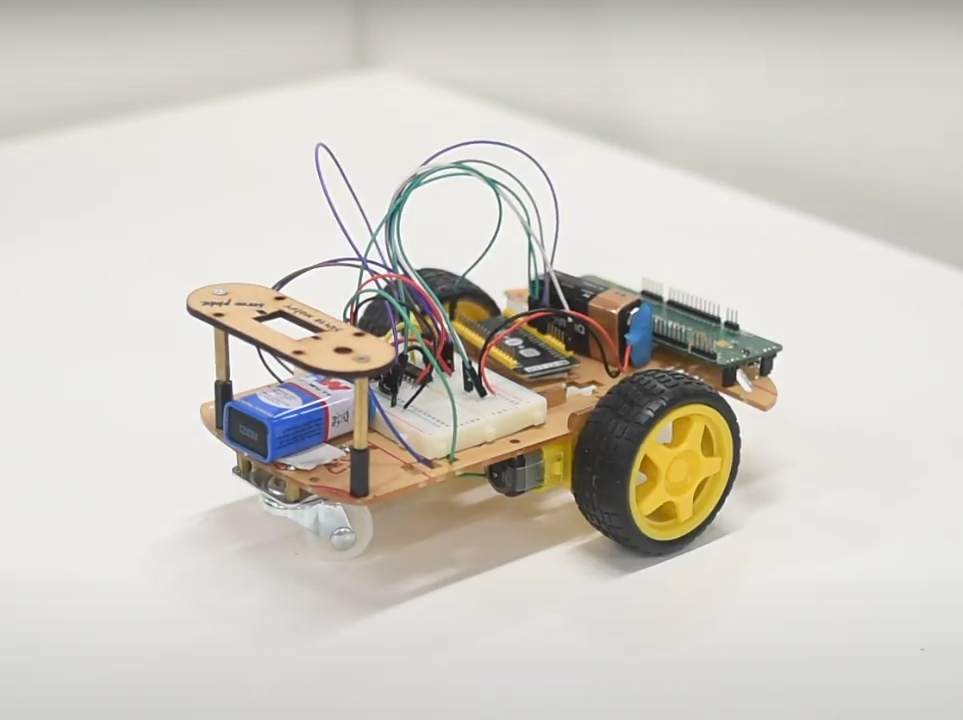
\includegraphics[width=0.8\linewidth]{./figs/UGV_components_1.png}
  \caption{UGV kit hardware}
  \label{UGV_kit_hardware}
\end{figure}
%\begin{columns}
%\column{1\textwidth}
%\end{columns}
\end{frame}

\section{UAV kit hardware}
\begin{frame}
\frametitle{UAV kit hardware}
\begin{figure}[h!]
  \centering
  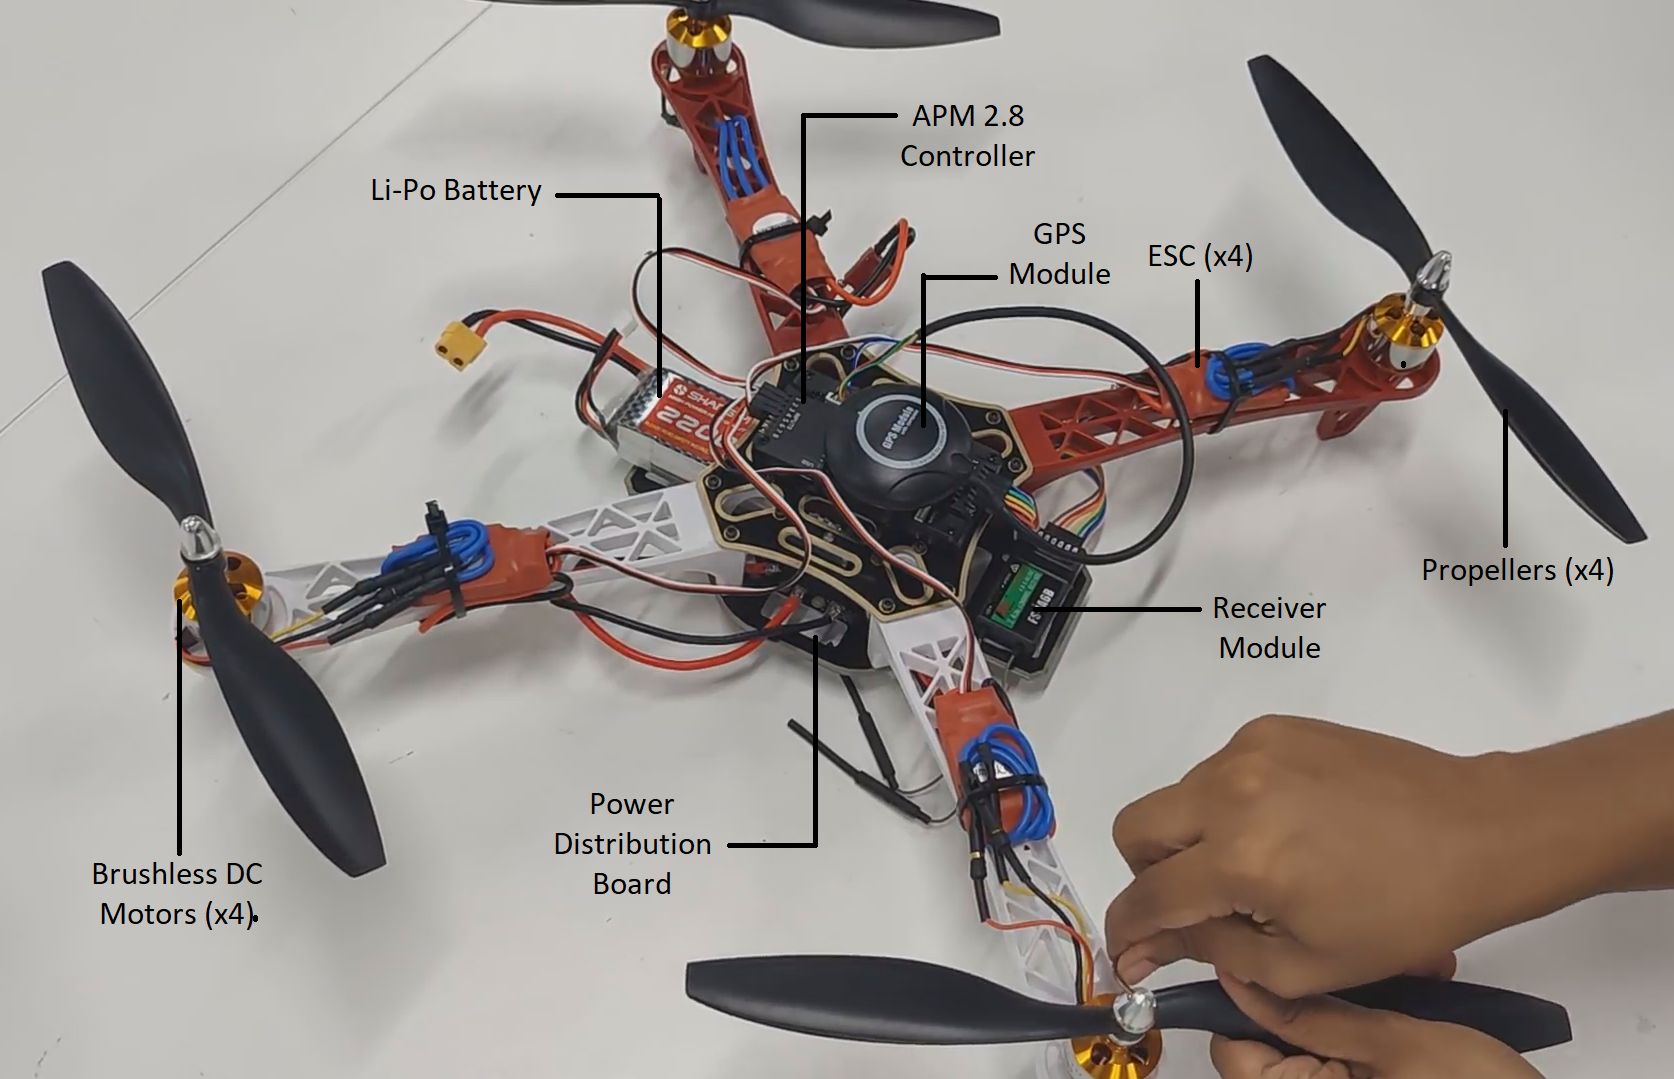
\includegraphics[width=0.9\linewidth]{./figs/UAV_components.png}
  \caption{UAV kit hardware}
  \label{fig:side3}
\end{figure}
%\begin{columns}
%\column{1\textwidth}
%\end{columns}
\end{frame}

\section{Controllers}
\begin{frame}
\frametitle{Controllers}
\begin{table}[H]
\centering
\resizebox{\textwidth}{!}{
\begin{tabular}{|l|c|c|c|}
\hline
\textbf{Parameters} & \textbf{Arduino Uno} & \textbf{Raspberry Pi 3B} & \textbf{ESP-32} \\ \hline
\textbf{Processor} & ATMega328P & \begin{tabular}[c]{@{}c@{}}Quad-core Broadcom \\ BCM2837 (4×Cortex-A53)\end{tabular} & \begin{tabular}[c]{@{}c@{}}Xtensa Dual-Core 32-bit \\ LX6 with 600 DMIPS\end{tabular} \\ \hline
\textbf{GPU} & - & \begin{tabular}[c]{@{}c@{}}Broadcom VideoCore IV \\ @ 250 MHz\end{tabular} & - \\ \hline
\textbf{Operating voltage} & 5V & 5V & 3.3V \\ \hline
\textbf{Clock speed} & 16 MHz & 1.2GHz & 26 MHz – 52 MHz \\ \hline
\textbf{System memory} & 2kB & 1 GB & \textless{}45kB \\ \hline
\textbf{Flash memory} & 32 kB & - & up to 128MB \\ \hline
\textbf{EEPROM} & 1 kB & - & - \\ \hline
\textbf{\begin{tabular}[c]{@{}l@{}}Communication \\ supported\end{tabular}} & \begin{tabular}[c]{@{}c@{}}IEEE 802.11 b/g/n\\ Bluetooth via Shield\end{tabular} & \begin{tabular}[c]{@{}c@{}}IEEE 802.11 b/g/n\\ Bluetooth, Ethernet Serial\end{tabular} & IEEE 802.11 b/g/n \\ \hline
\textbf{\begin{tabular}[c]{@{}l@{}}Development \\ environments\end{tabular}} & Arduino IDE & \begin{tabular}[c]{@{}c@{}}Any linux \\ compatible IDE\end{tabular} & Arduino IDE, Lua Loader \\ \hline
\textbf{\begin{tabular}[c]{@{}l@{}}Programming \\ language\end{tabular}} & Embedded C, C++ & \begin{tabular}[c]{@{}c@{}}Python, C, C++, Java,\\ Scratch, Ruby\end{tabular} & Embedded C, C++ \\ \hline
\textbf{I/O Connectivity} & SPI I2C UART GPIO & \begin{tabular}[c]{@{}c@{}}SPI DSI UART \\ SDIOCSI GPIO\end{tabular} & UART, GPIO \\ \hline
\end{tabular}
}
\caption{Comparison between Arduino Uno, Raspberry Pi 3B and ESP-32}
\end{table}
\end{frame}

\section{Controllers (Vaman)}
\begin{frame}
\frametitle{Controllers (Vaman)}
\begin{columns}
	\column{0.5\textwidth}
	\begin{itemize}
		\item On-board dual processor (ARM + FPGA)
		\item On-board WiFi/BT/BLE connectivity with ESP32
		\item $\mu$SD card support
		\item On-board inertial measurement unit
		\item On-board BMO055 smart fusion sensor
		\item On-board DPS310 provides pressure, humidity and temperature monitoring
	\end{itemize}

	\column{0.5\textwidth}
	\begin{figure}[h!]
  		\centering
  		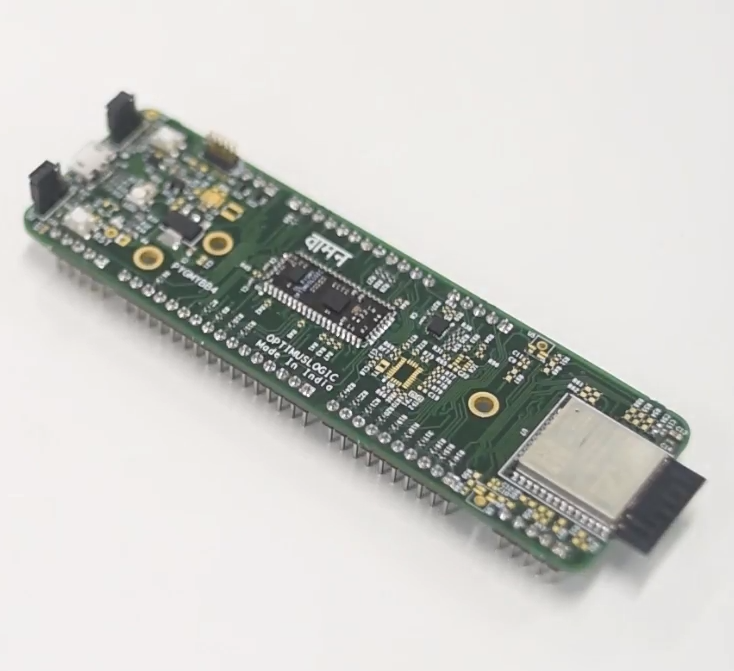
\includegraphics[width=0.8\linewidth]{./figs/Vaman.png}
  		\caption{Vaman - Pygmy BB4}
  		\label{Vaman}
	\end{figure}
\end{columns}
\end{frame}

\section{Motor control using PWM}
\begin{frame}
\frametitle{Motor control using PWM}
\begin{itemize}
	\item A pulse width modulation speed control system works by sending a series of "ON-OFF" pulses
to the motor. The frequency of square wave is kept constant while varying the duty cycle (the
fraction of time that the output voltage is "ON" compared to when it is "OFF").
	\item By changing the width of the ON duration, one can control the average DC voltage applied to
the motor. The below equation (\ref{eq1}) gives the relation between the Duty cycle ($D$) and the average voltage:

\begin{align}
V_{dc}&={\frac {1}{T}}\int _{0}^{T}v_{PWM}(t)\,dt  \label{eq1} \\
V_{dc} &= {\frac {1}{T}}\left(\int _{0}^{DT}v_{\text{max}}\,dt+\int _{DT}^{T}v_{\text{min}}\,dt\right) \nonumber \\ \nonumber
&={\frac {1}{T}}\left(D\cdot T\cdot v_{\text{max}}+T\left(1-D\right)v_{\text{min}}\right)\\ \nonumber
&=D\cdot v_{\text{max}}+\left(1-D\right)v_{\text{min}} 
\end{align}
\end{itemize}
\end{frame}

\section{Motor control using PWM 1}
\begin{frame}
\frametitle{Motor control using PWM \small{(Continued)}}
\begin{figure}[t!]
    \centering
    \begin{subfigure}[t]{0.5\textwidth}
        \centering
        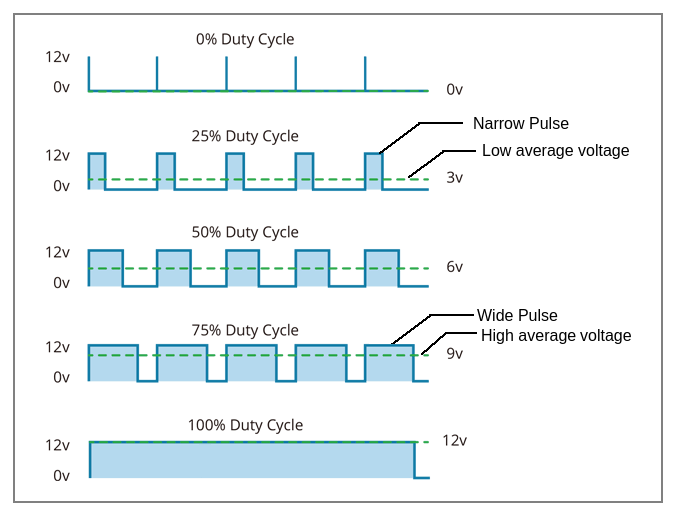
\includegraphics[width = 7cm]{./figs/PWM_speed_control.png}
        \caption{PWM speed control}
    \end{subfigure}%
    ~ 
    \begin{subfigure}[t]{0.5\textwidth}
        \centering
        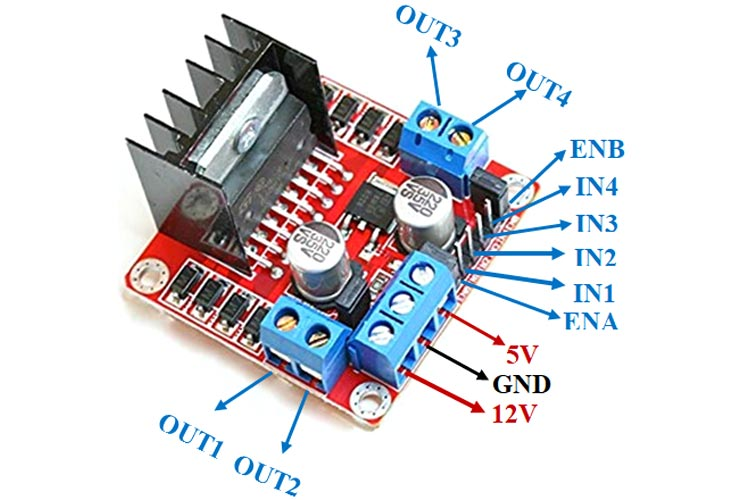
\includegraphics[width = 4.5cm]{./figs/Motor_driver_L298.jpg}
        \caption{Dual motor driver module (L298N)}
    \end{subfigure}

\end{figure} 	
\end{frame}




\section{ESP32 Based Application 1}
\begin{frame}
\frametitle{ESP32 Based Application-1}
\begin{columns}
	\column{0.95\textwidth}
	\begin{figure}[h!]
  		\centering
  		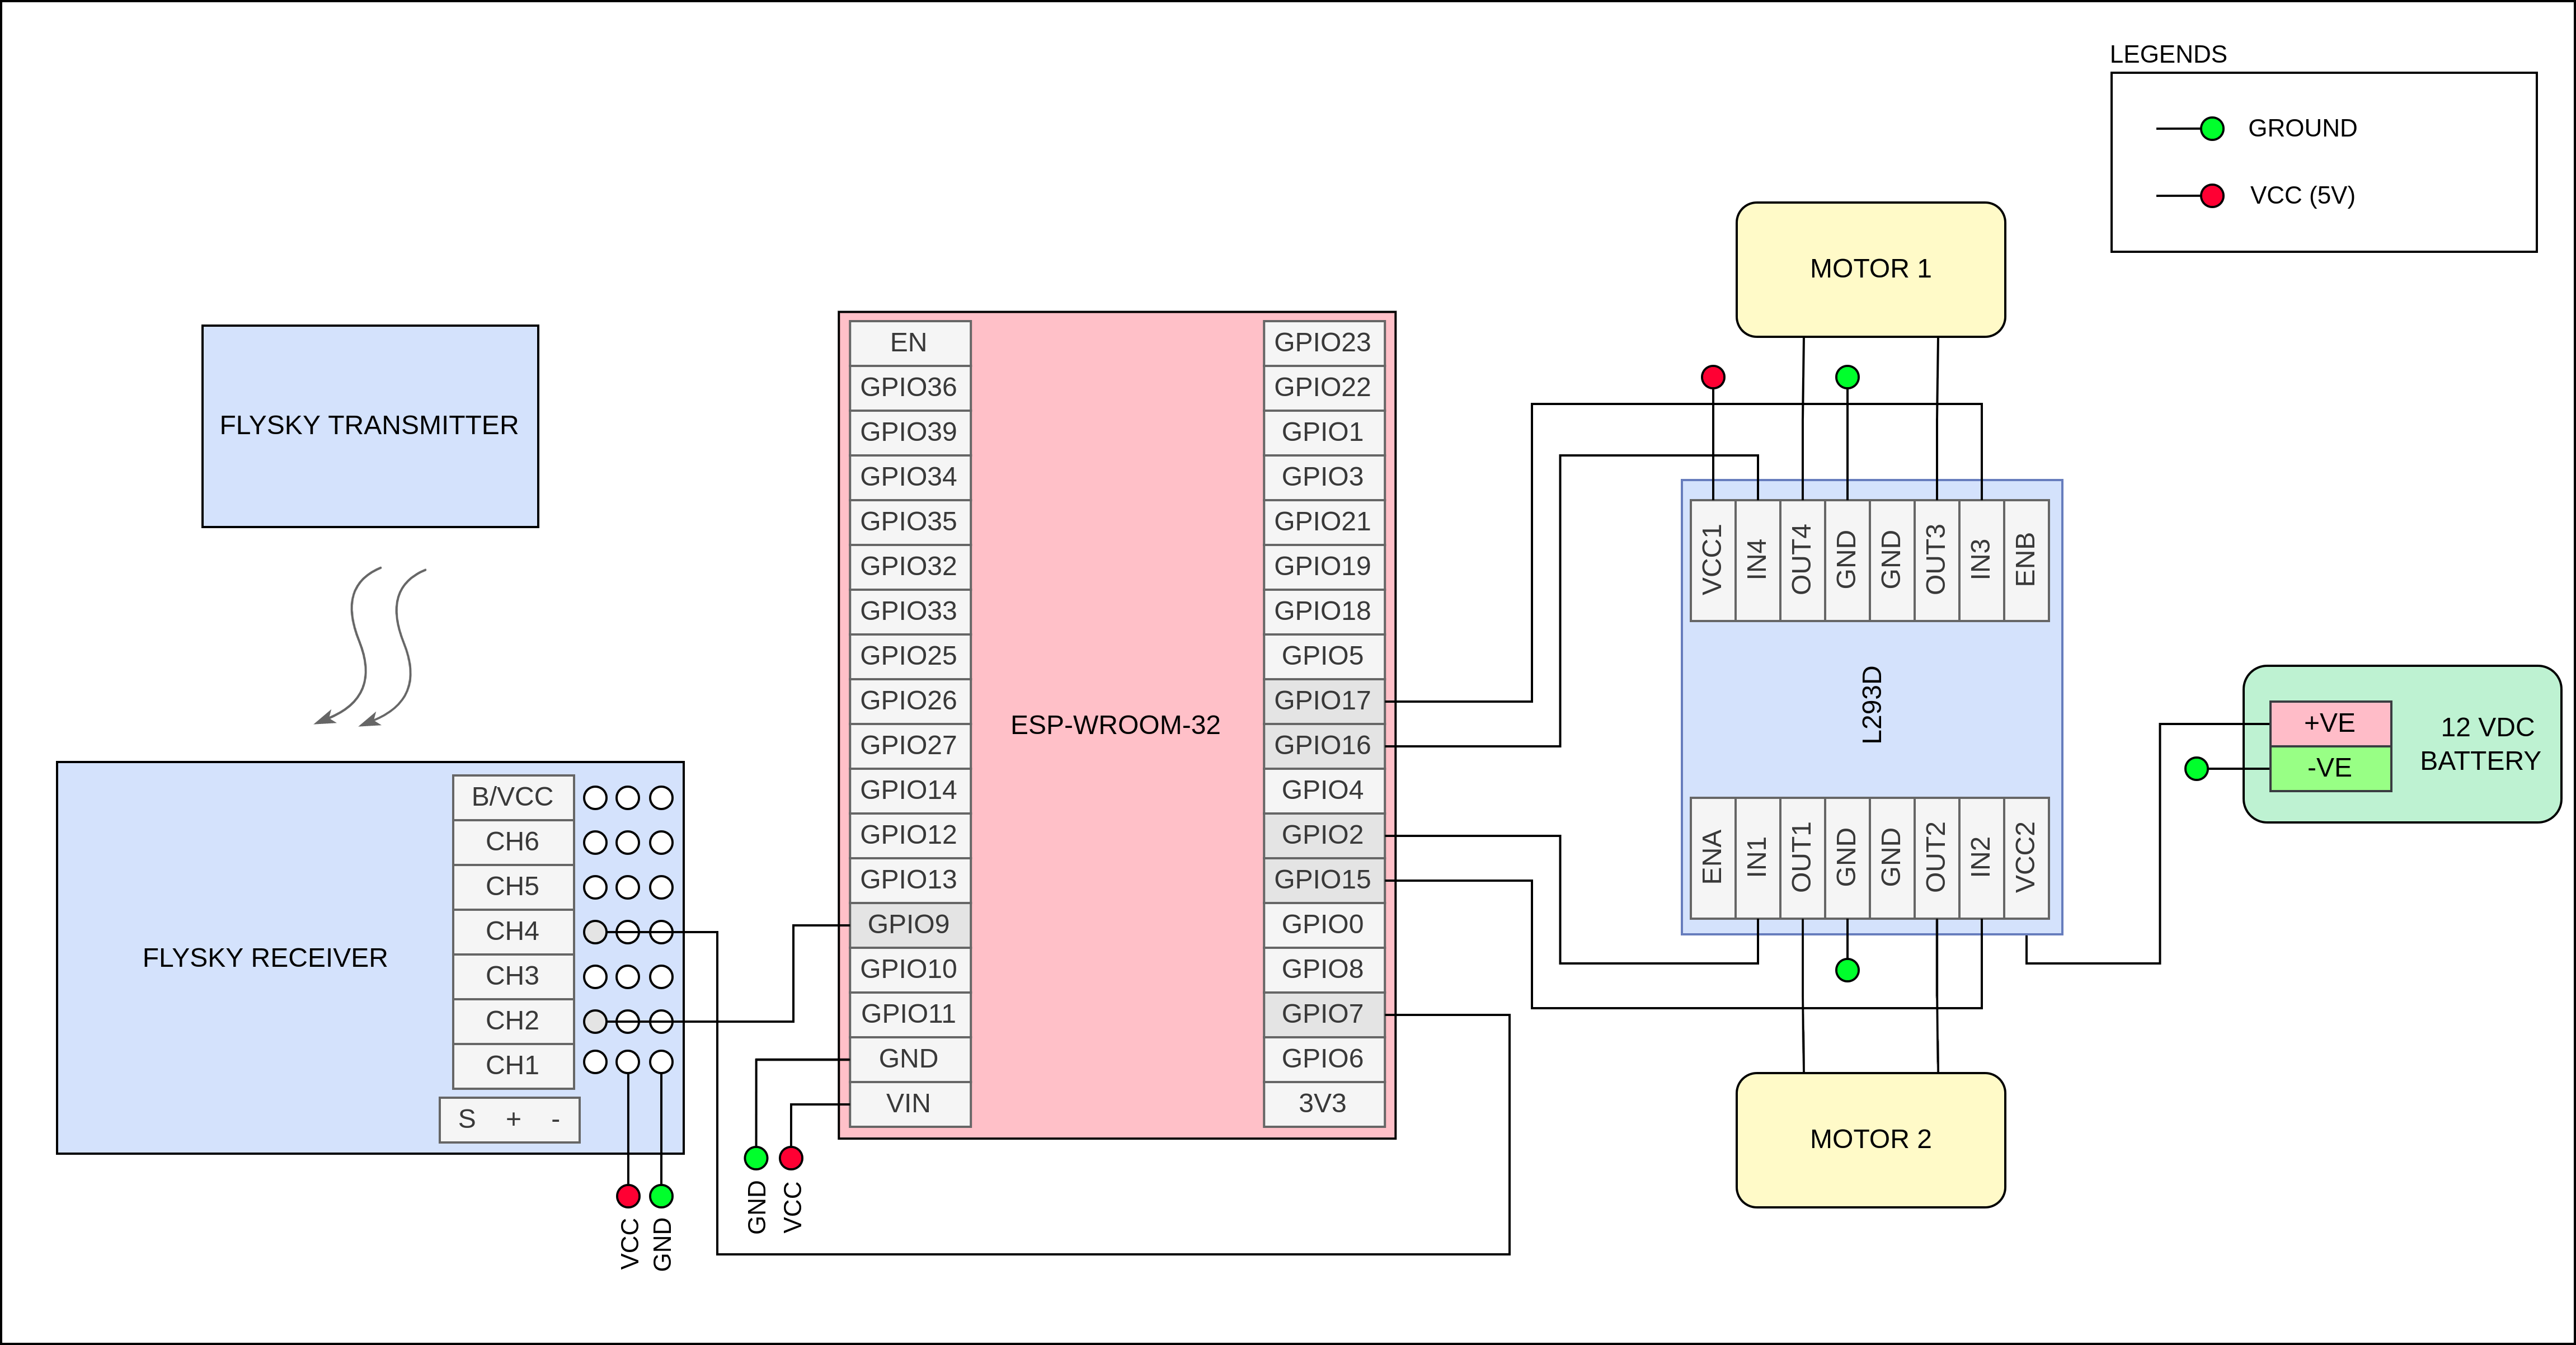
\includegraphics[width=\linewidth]{./figs/Wiring_UGV_flysky.png}
  		\caption{UGV Navigation using Fly-sky transmitter \& receiver (ESP32)}
  		\label{Wiring_UGV_flysky}
	\end{figure}
\end{columns}
\end{frame}

\section{ESP32 Based Application 2}
\begin{frame}
\frametitle{ESP32 Based Application-2}
\begin{columns}
	\column{0.8\textwidth}
	\begin{figure}[h!]
  		\centering
  		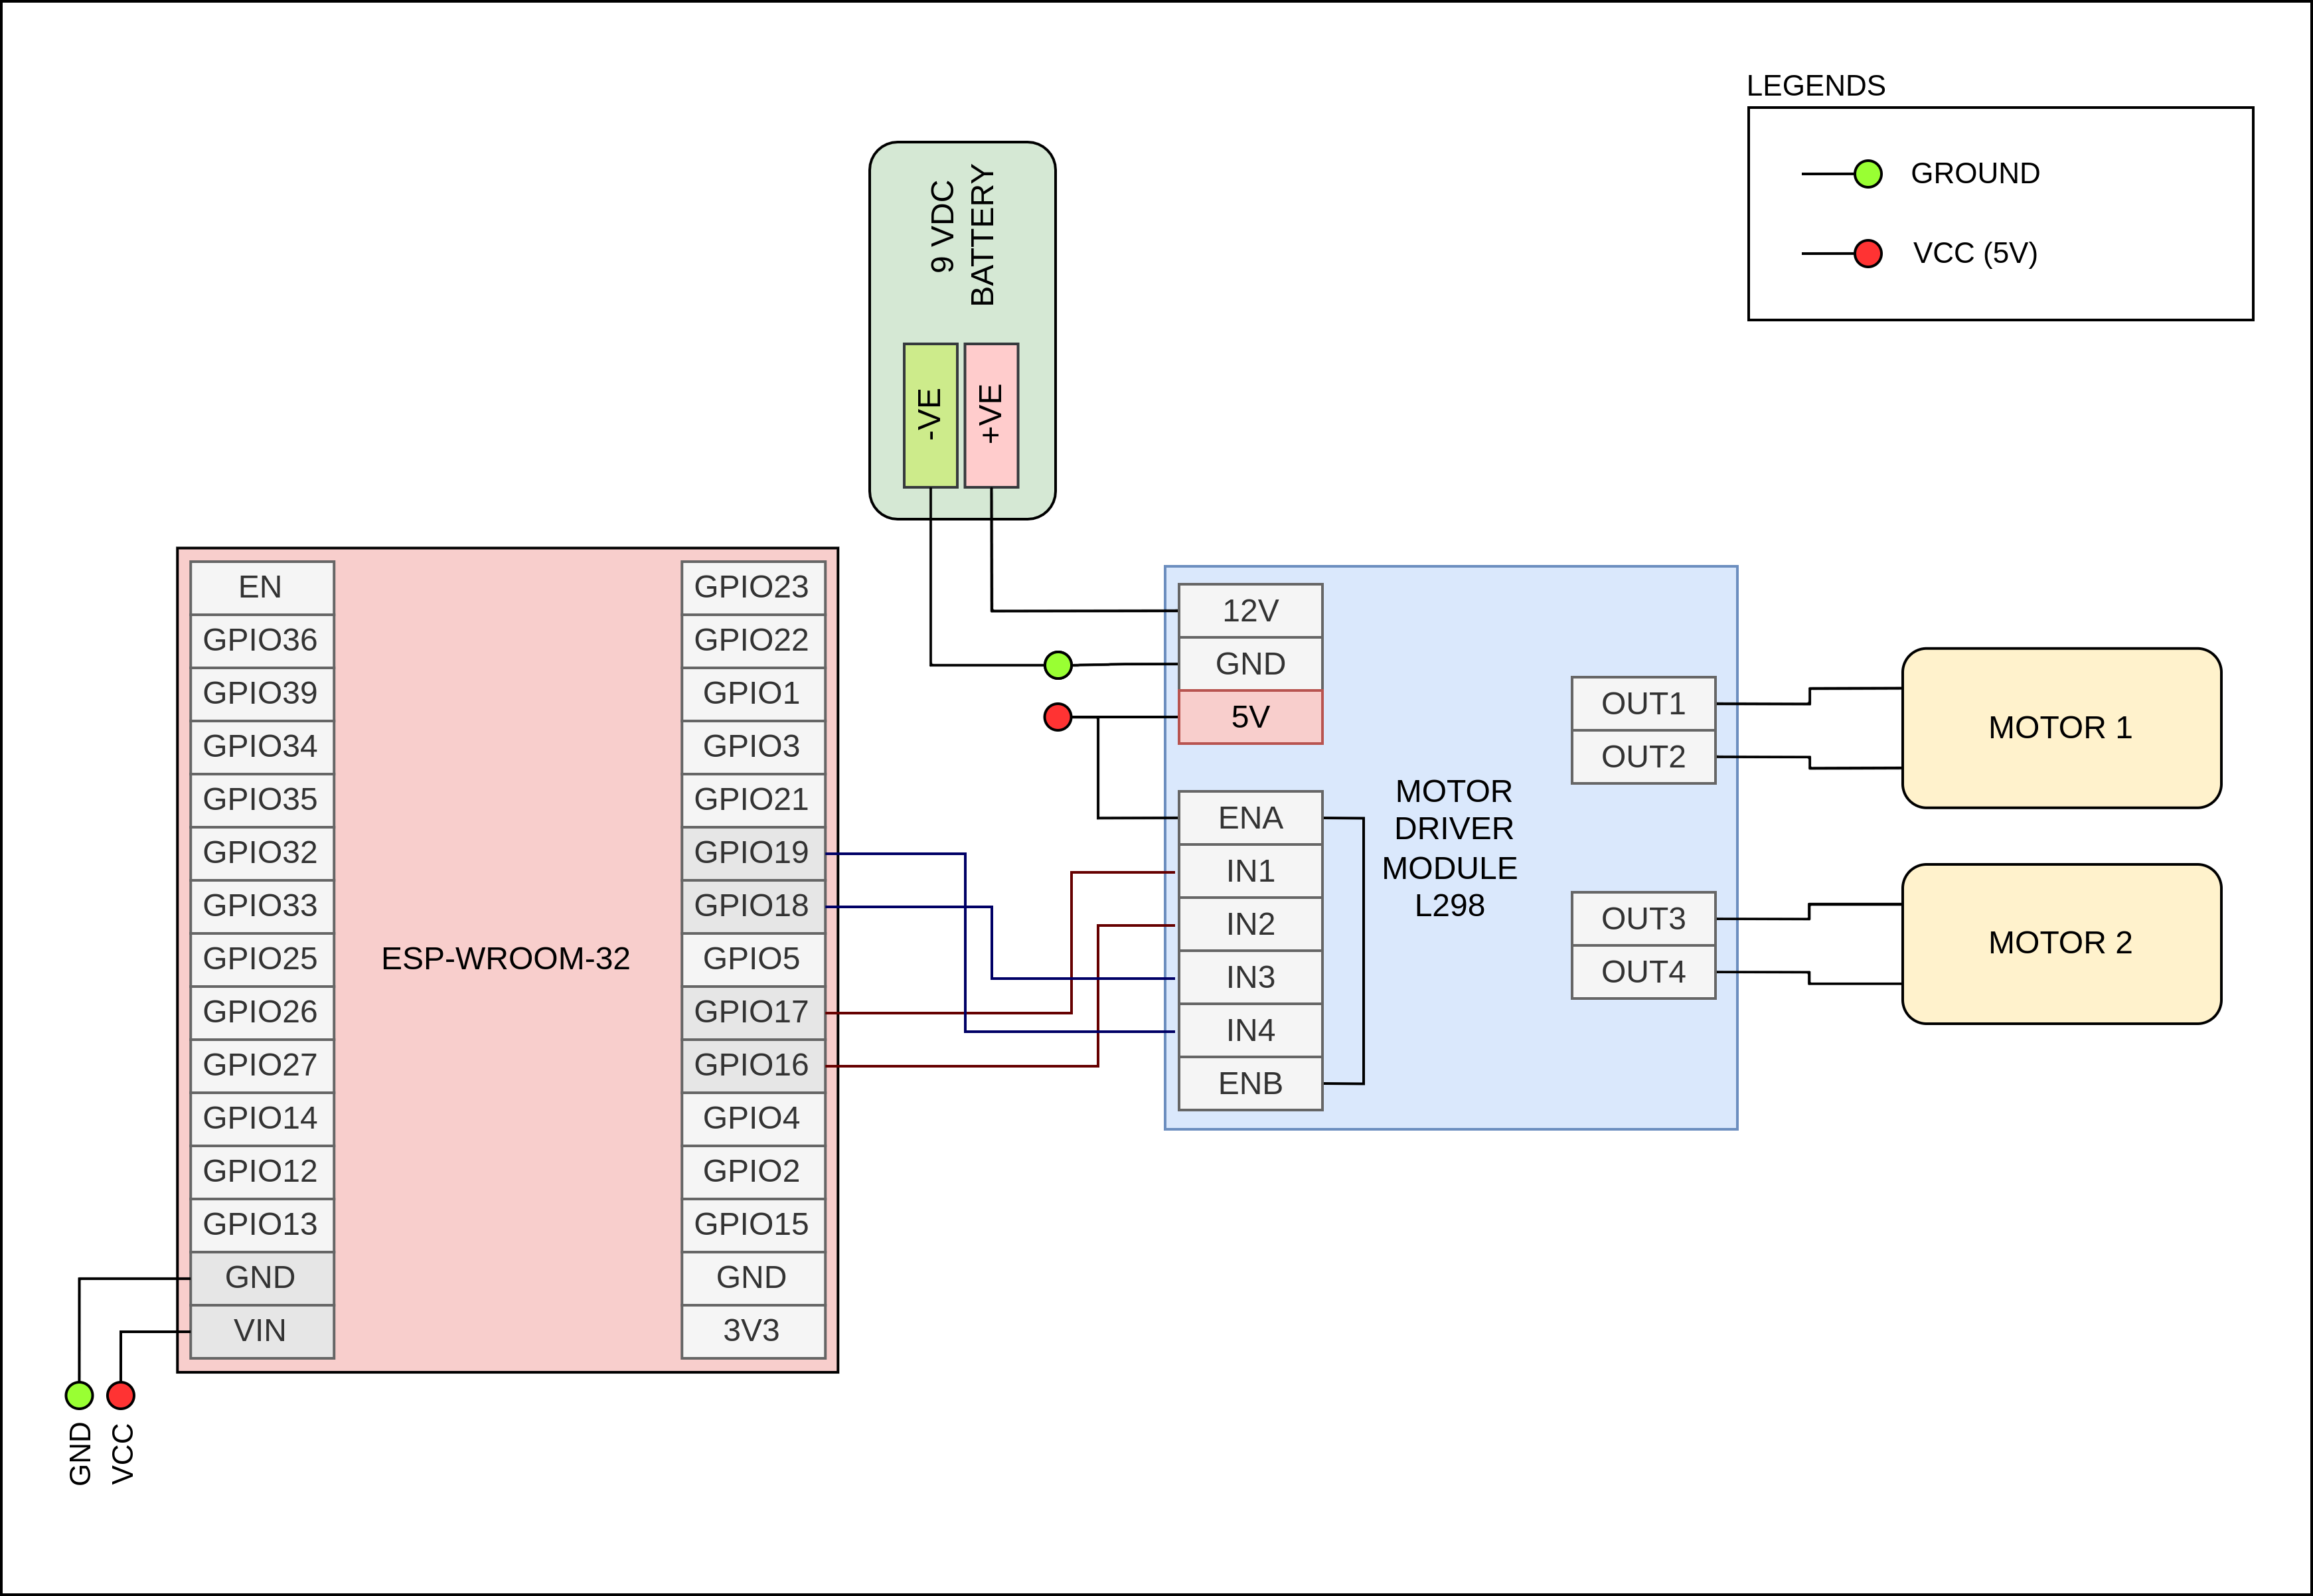
\includegraphics[width=\linewidth]{./figs/Wiring_UGV_speech.png}
  		\caption{UGV Navigation using Android phone (ESP32)(Manual and Speech)}
  		\label{Wiring_UGV_speech}
	\end{figure}
\end{columns}
\end{frame}

\section{ESP32 Based Application 3}
\begin{frame}
\frametitle{ESP32 Based Application-3}
\begin{columns}
	\column{0.95\textwidth}
	\begin{figure}[h!]
  		\centering
  		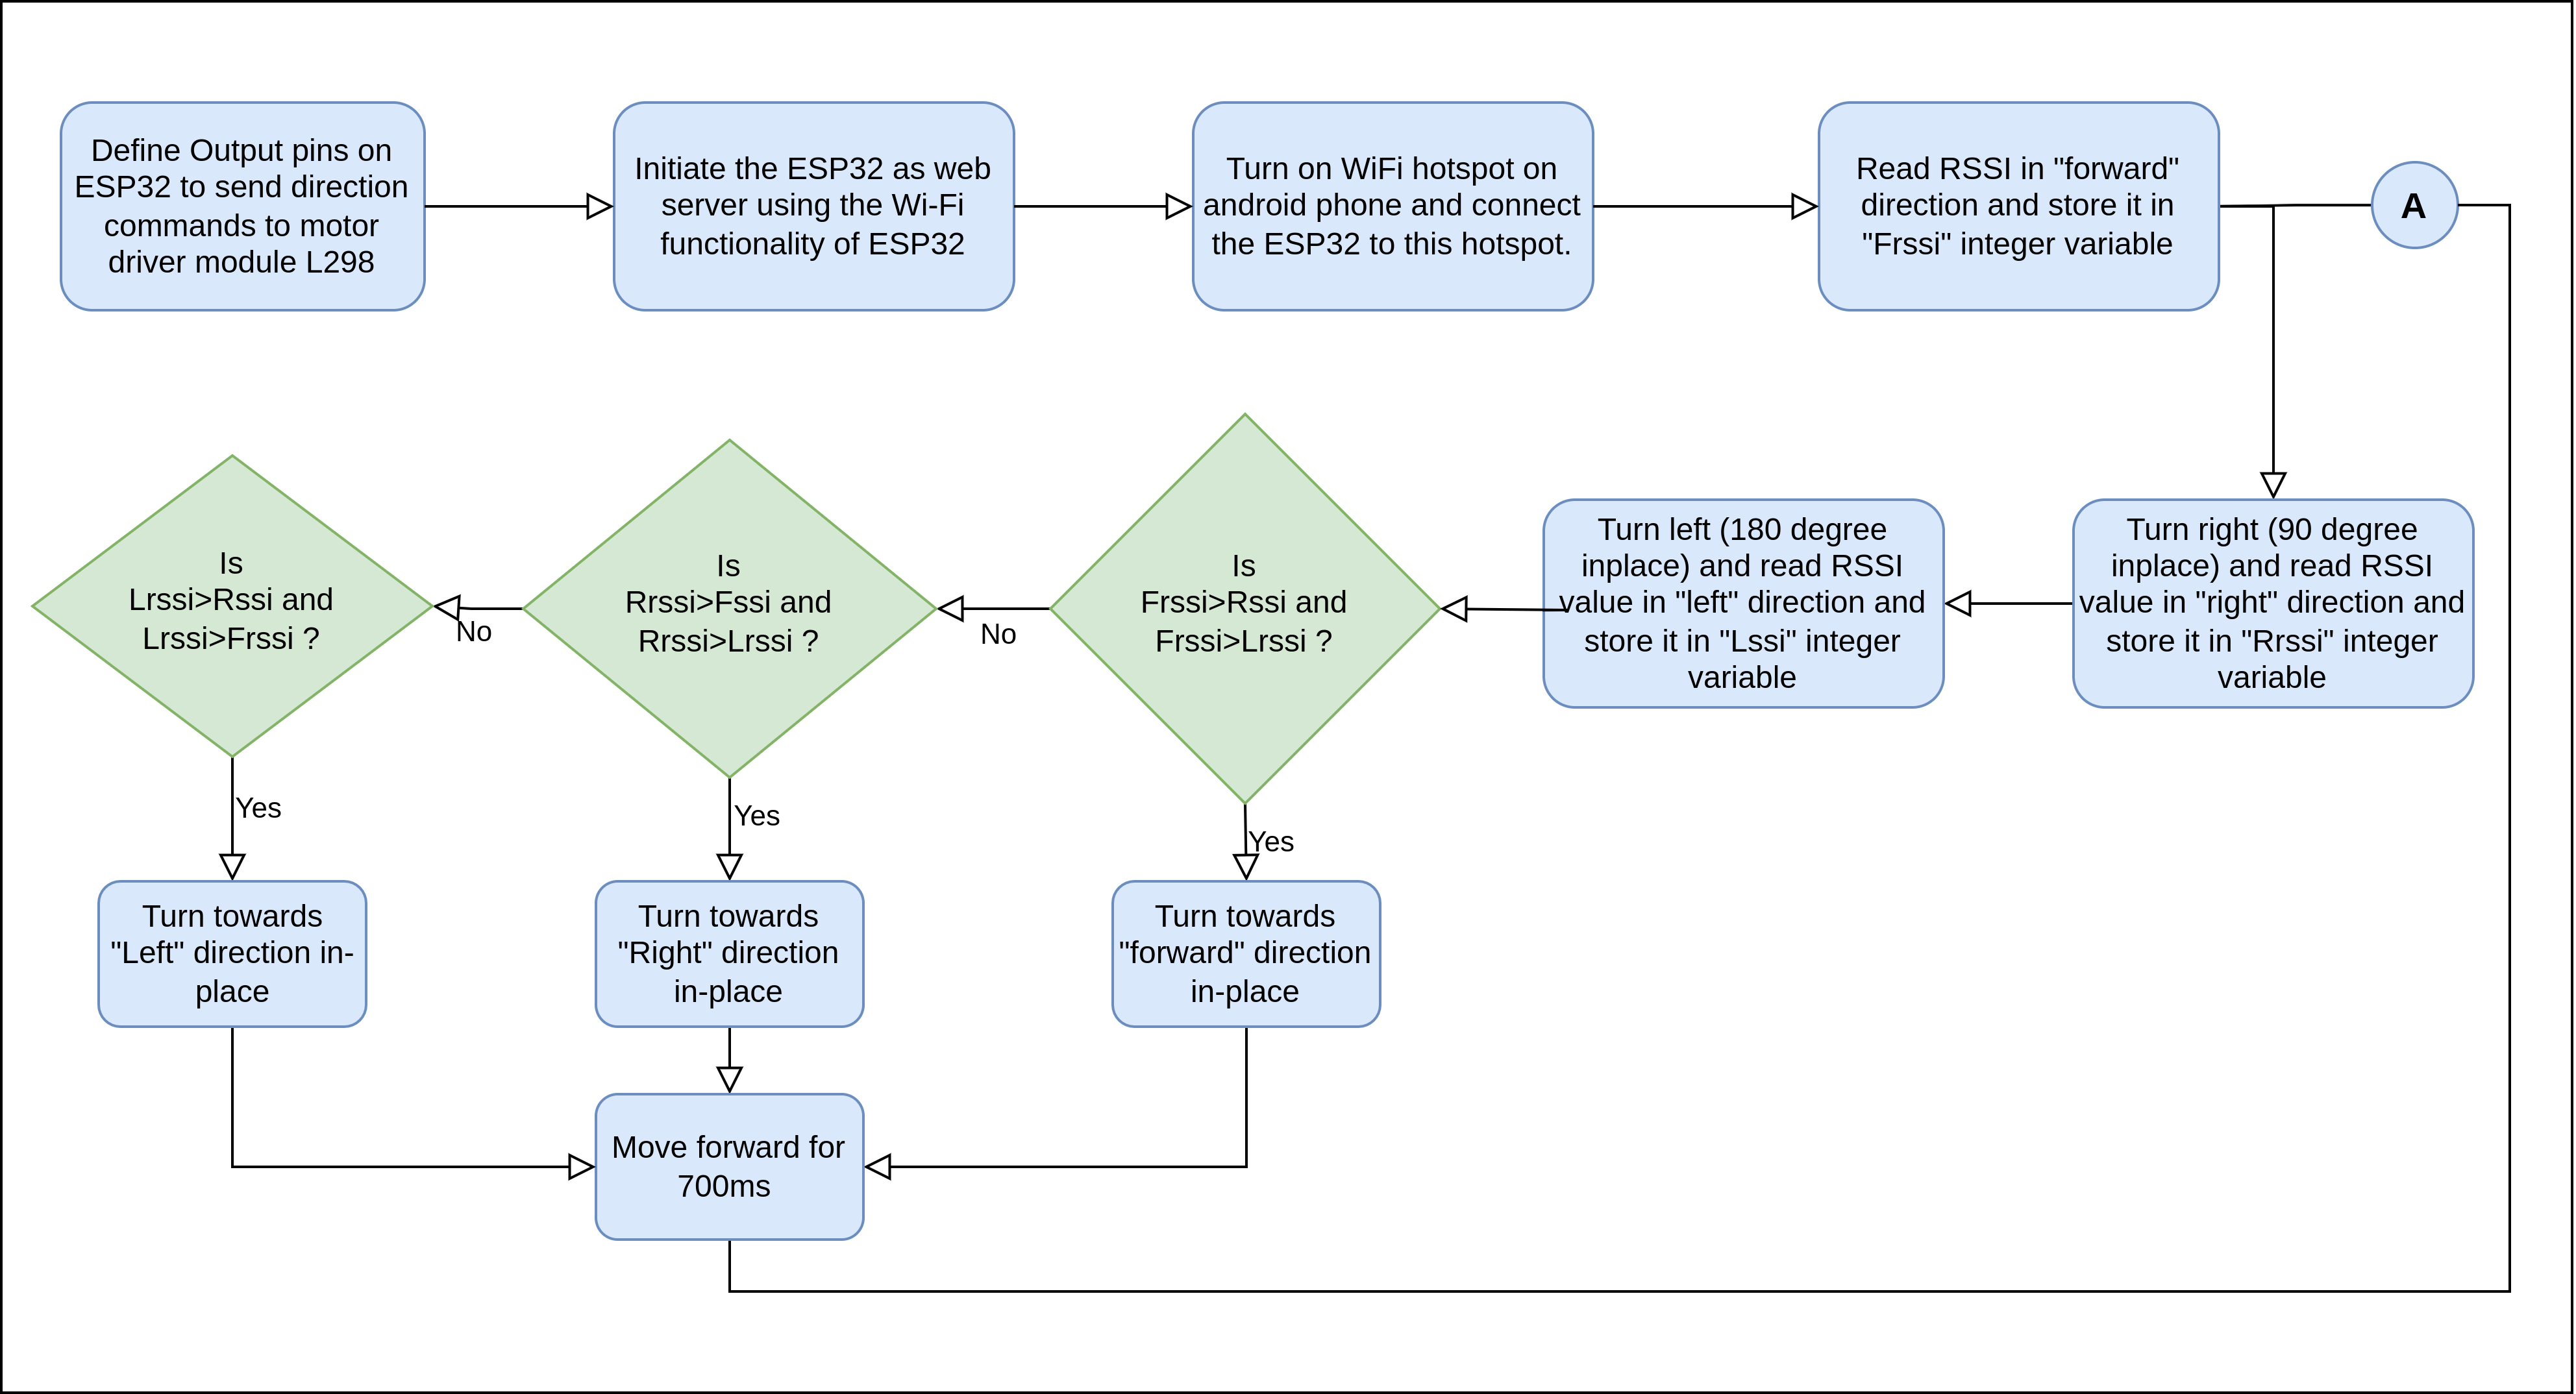
\includegraphics[width=\linewidth]{./figs/Flow_UGV_beacon.png}
  		\caption{UGV beacon tracking}
  		\label{Flow_UGV_beacon}
	\end{figure}
\end{columns}
\end{frame}

\section{ESP32 Based Application 4}
\begin{frame}
\frametitle{ESP32 Based Application-4}
\begin{columns}
	\column{0.95\textwidth}
	\begin{figure}[h!]
  		\centering
  		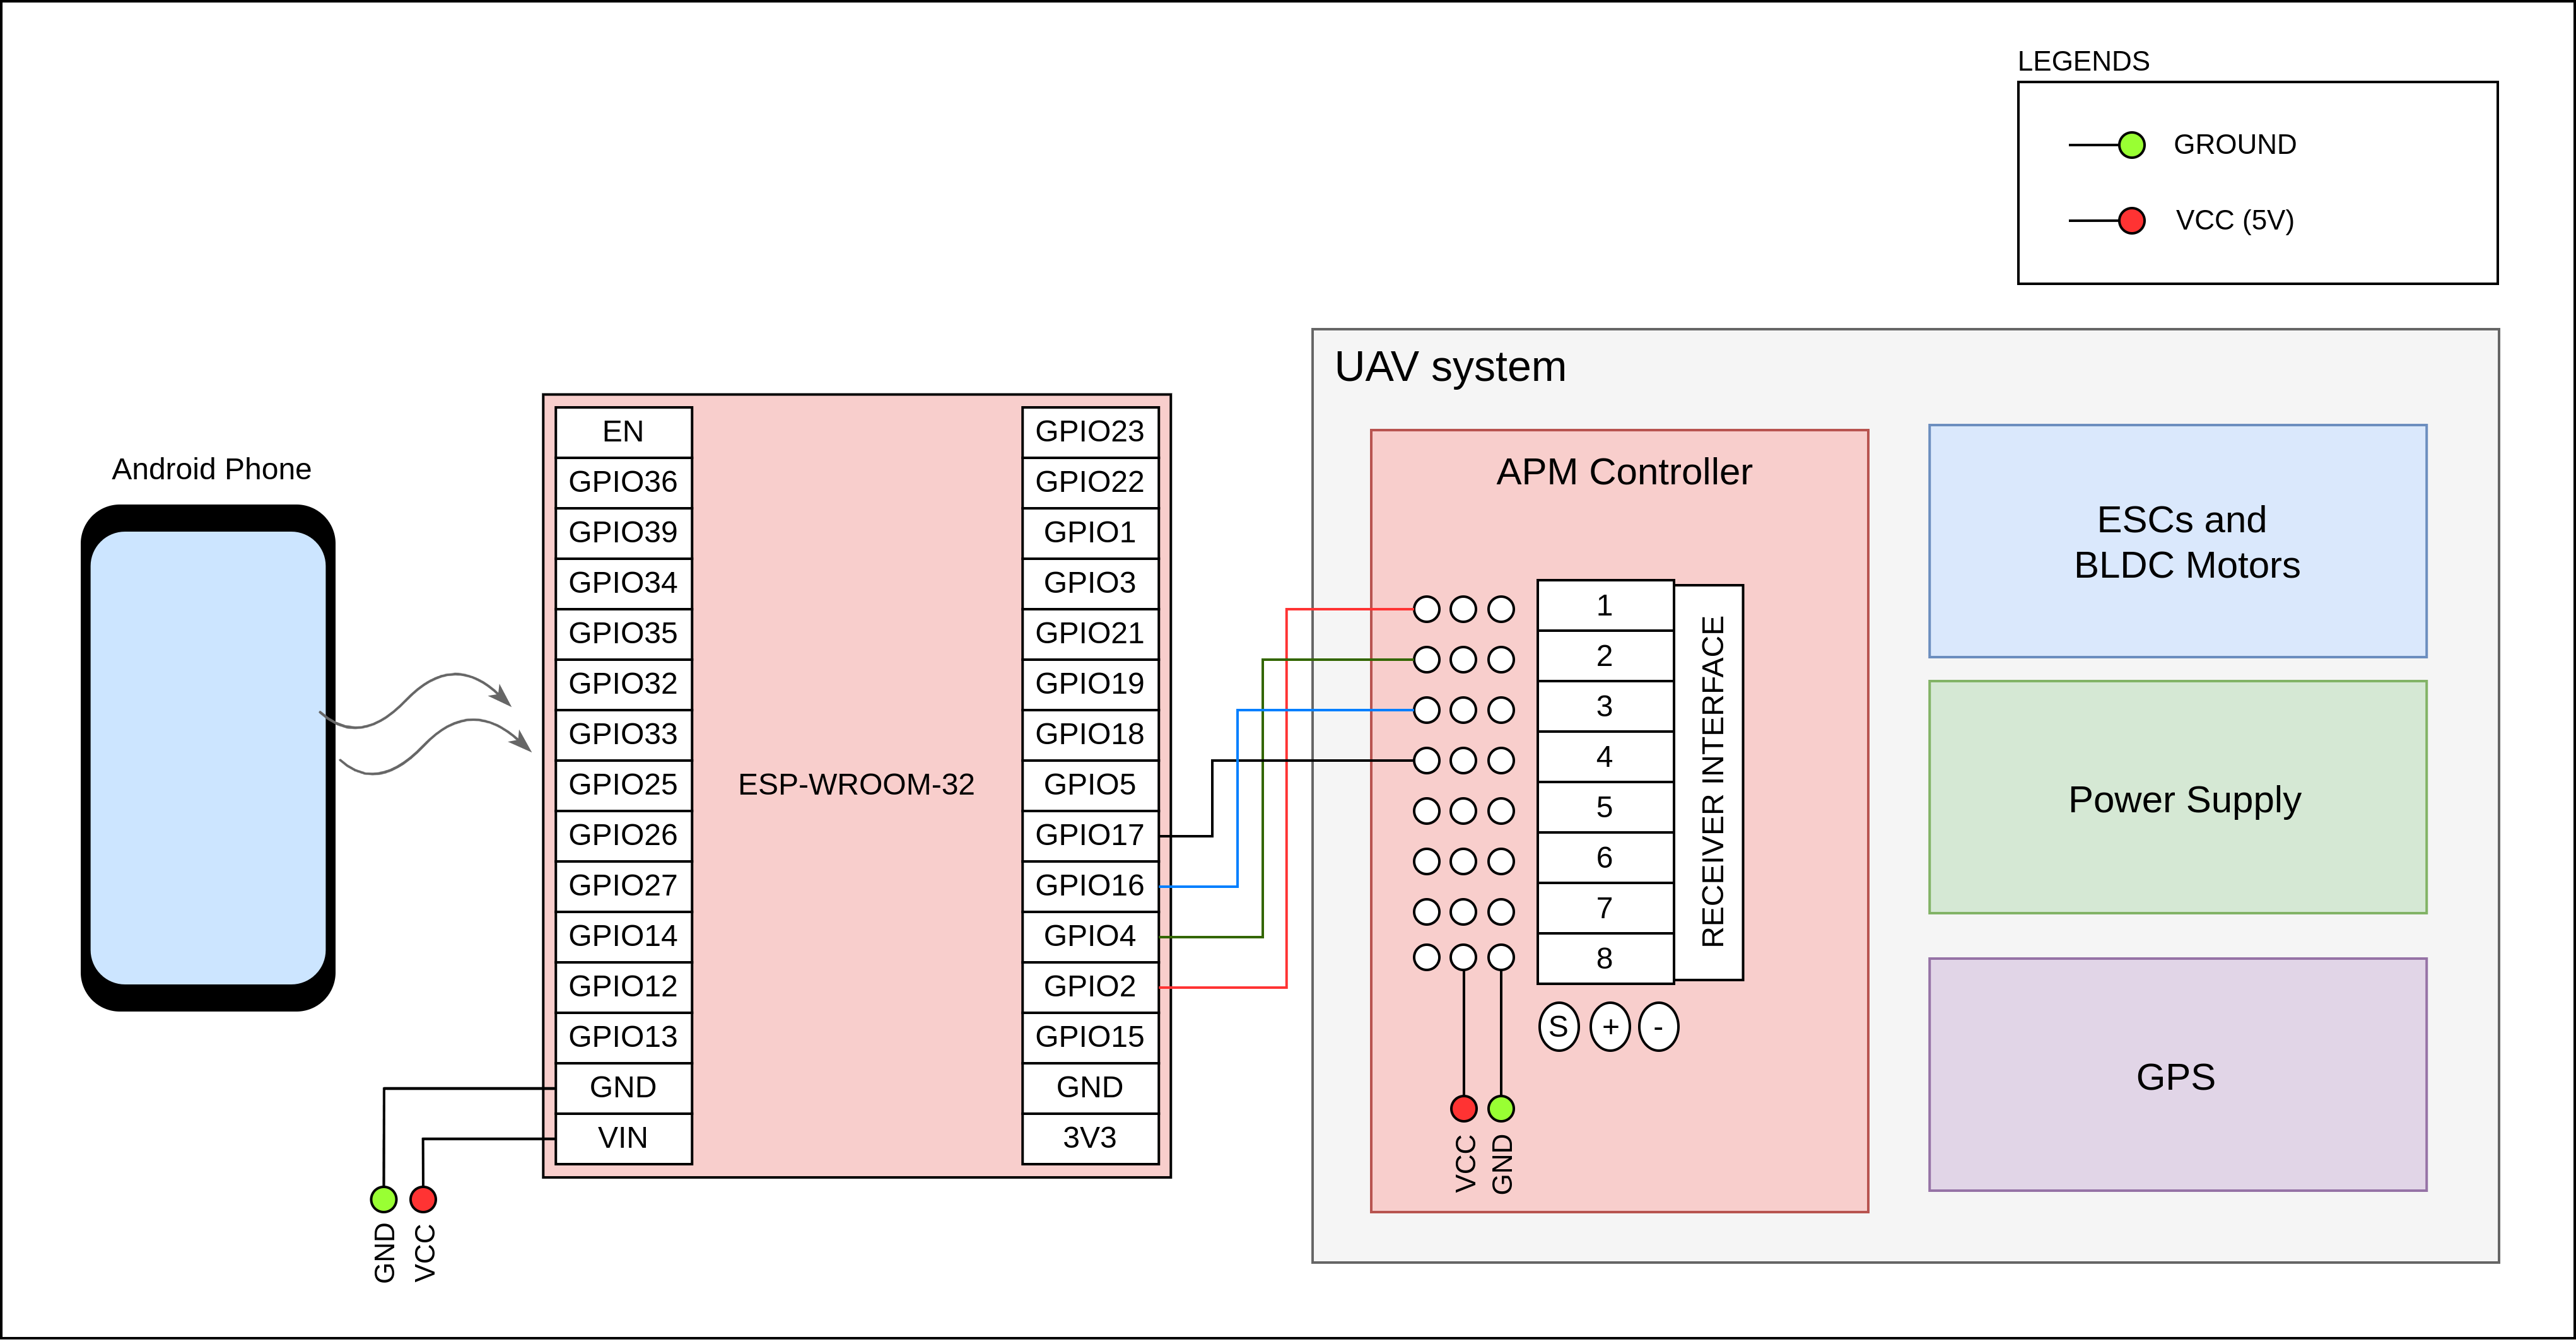
\includegraphics[width=\linewidth]{./figs/Wiring_UAV_ESP32_commlink.png}
  		\caption{UAV Navigation using ESP32 and Android phone}
  		\label{Wiring_UAV_ESP32_commlink}
	\end{figure}
\end{columns}
\end{frame}

\section{Vaman Based Application 1}
\begin{frame}
\frametitle{Vaman Based Application-1}
\begin{columns}
	\column{0.75\textwidth}
	\begin{figure}[h!]
  		\centering
  		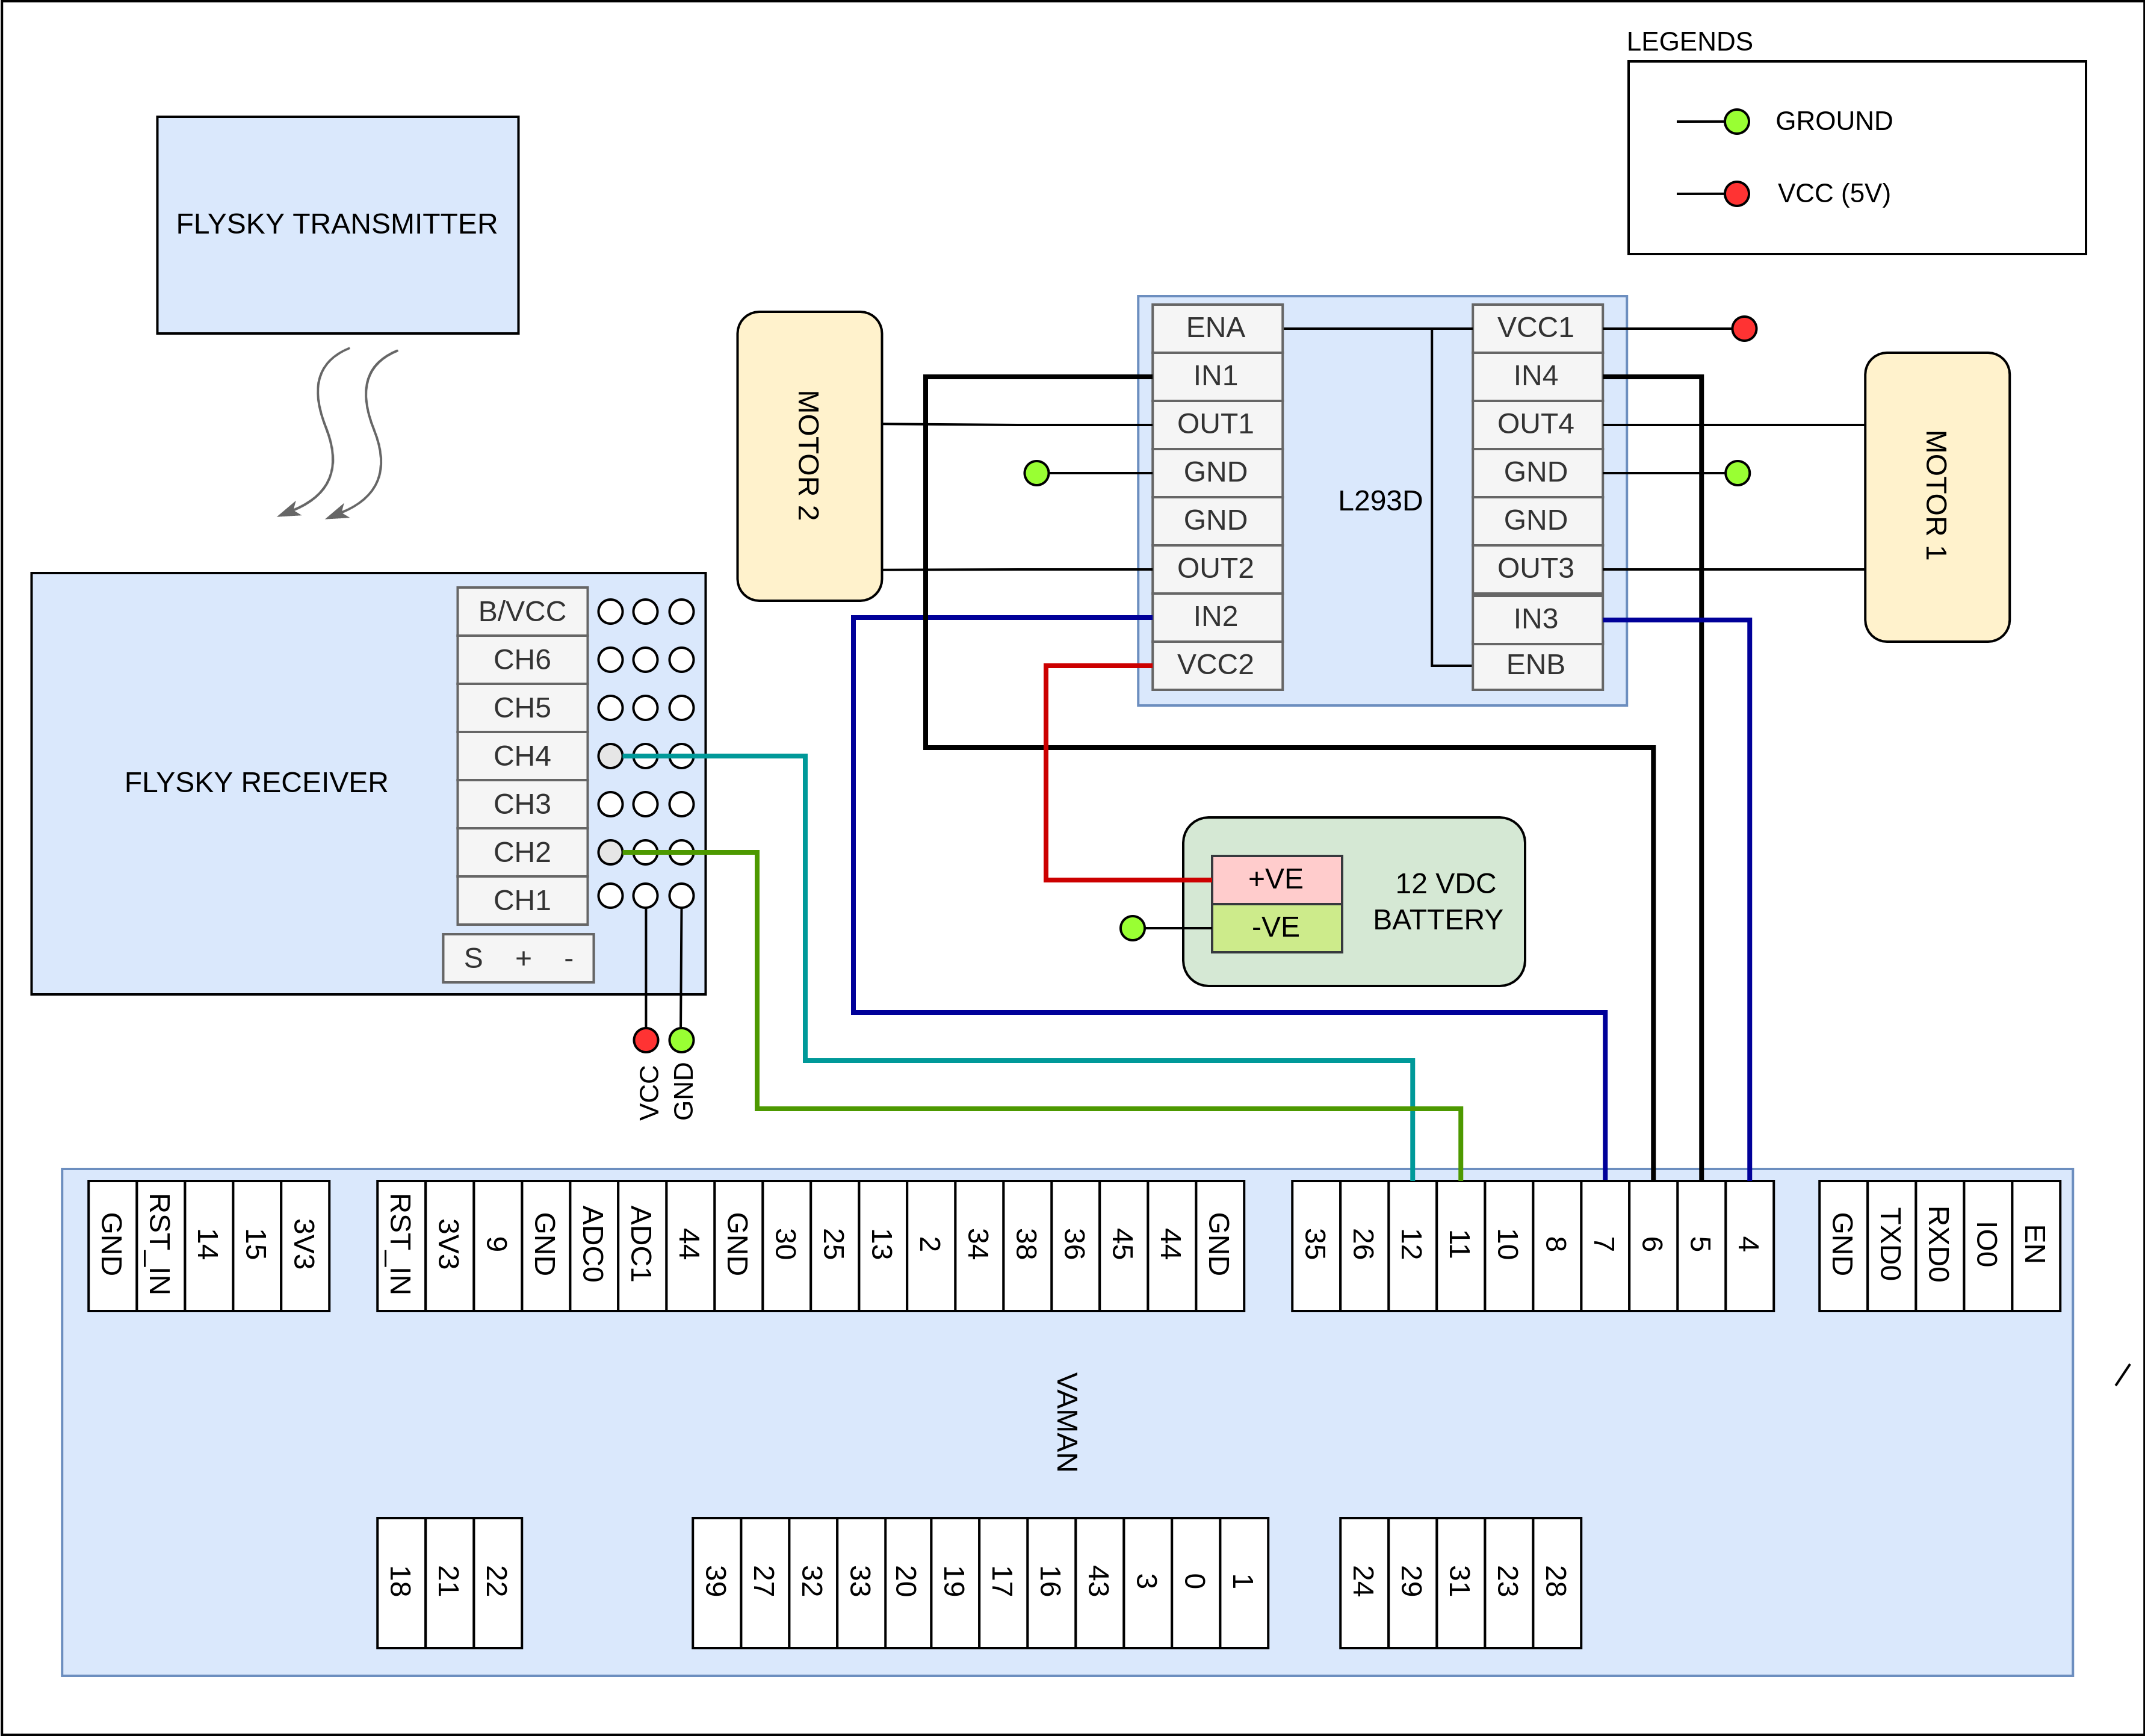
\includegraphics[width=\linewidth]{./figs/Wiring_UGV_flysky_Vaman.png}
  		\caption{UGV Navigation using Fly-sky transmitter \& receiver (Vaman)}
  		\label{Wiring_UGV_flysky_Vaman}
	\end{figure}
\end{columns}
\end{frame}

\section{Vaman Based Application 2}
\begin{frame}
\frametitle{Vaman Based Application-2}
\begin{columns}
	\column{0.75\textwidth}
	\begin{figure}[h!]
  		\centering
  		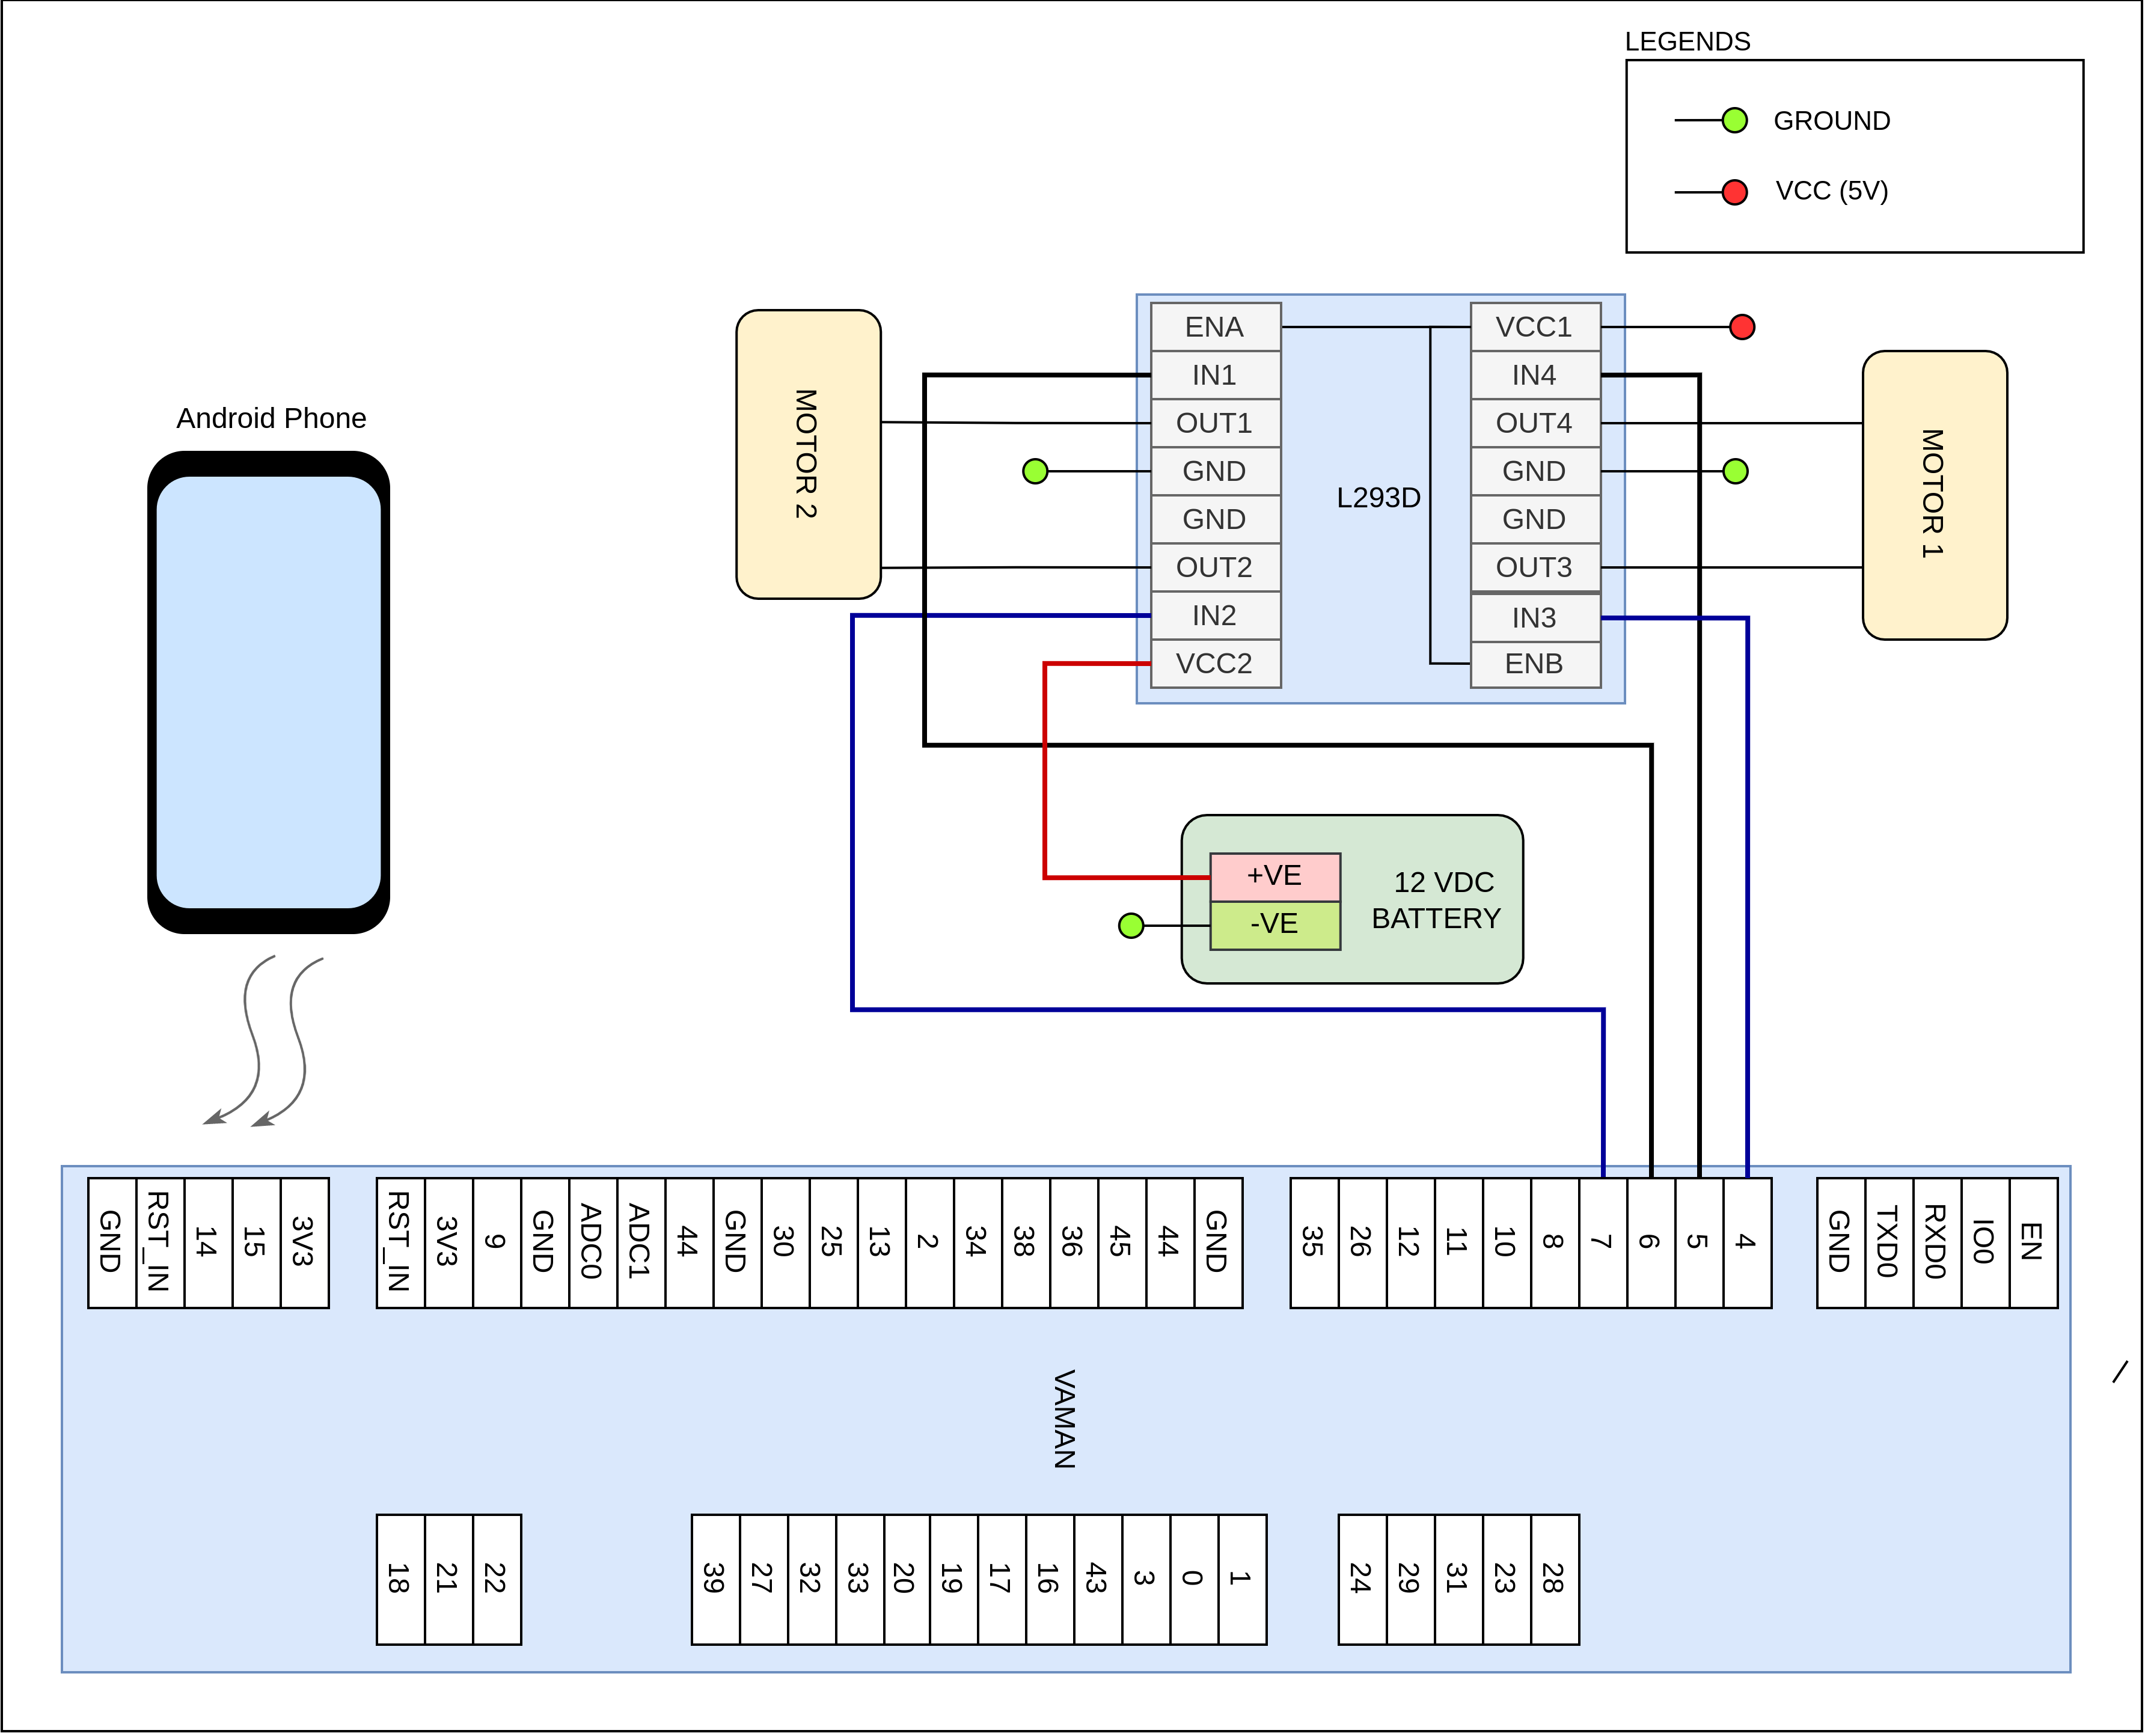
\includegraphics[width=\linewidth]{./figs/Wiring_UGV_phone_vaman.png}
  		\caption{UGV Navigation using Android phone (Vaman)}
  		\label{Wiring_UGV_phone_vaman}
	\end{figure}
\end{columns}
\end{frame}

\section{SATCOM for UAV Communication}
\begin{frame}{SATCOM for UAV Communication}
\begin{itemize}
	\item UAVs can utilise satellite communication (SATCOM) to send and receive data without having to send it back to the operator, as well as for remote access and control.
	\item Convinced by the potential of 5G, Satellite industry has shown increased interest and participation in 3GPP to integrate satellite infrastructure with terrestrial network of 5G
	\item Figure \ref{Conventional_5G} shows a typical 5G terrestrial network:
	\begin{figure}[h!]
  		\centering
  		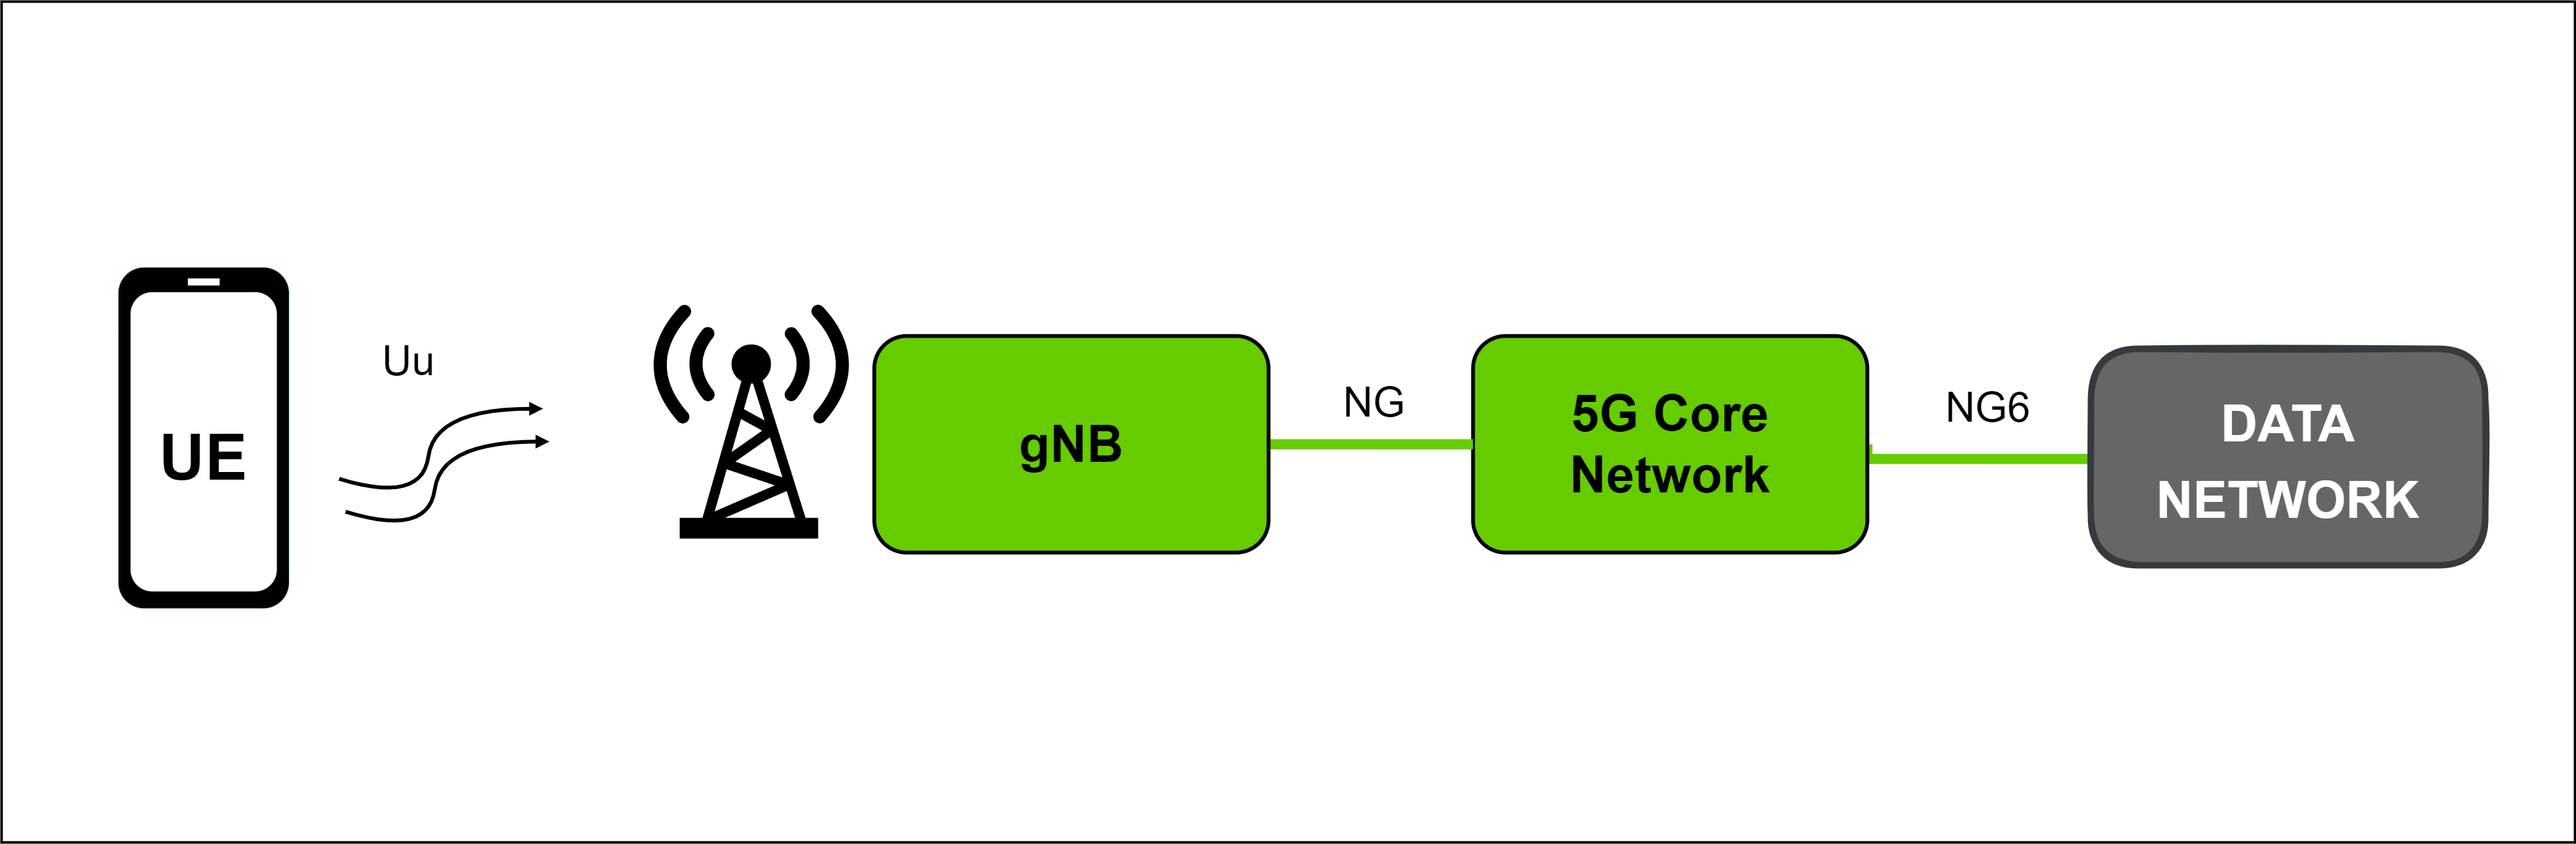
\includegraphics[width=0.9\linewidth]{./figs/Conventional_5G.png}
  		\caption{Terrestrial 5G-NR system}
  		\label{Conventional_5G}
	\end{figure}
\end{itemize}
\end{frame} 

\section{SATCOM for UAV Communication}
\begin{frame}{SATCOM for UAV \small{(Continued})}
\begin{itemize}
	\item In certain scenarios, our user equipment (in our case, a UAV) might not be reachable from the nearby gNB.(for instance, in isolated locations such as mountains, jungles, etc.)
	\item SATCOM provides a non-terrestrial network infrastructure, enabling communication with such
remote devices.
	\item Latest advancements in the satellite communications have overcome previous constraints. 
 \item New generation of Low Earth Orbit (LEO) constellations have lessened satellite communications latency
\item Technological improvements in Geostationary (GEO) satellites have provided high throughput and increased the reliability of GEO satellites.
\end{itemize}
\end{frame} 

\section{Transparent satellite based NG-RAN architecture}
\begin{frame}{Transparent satellite based NG-RAN architecture}
    \begin{figure}[h!]
  		\centering
  		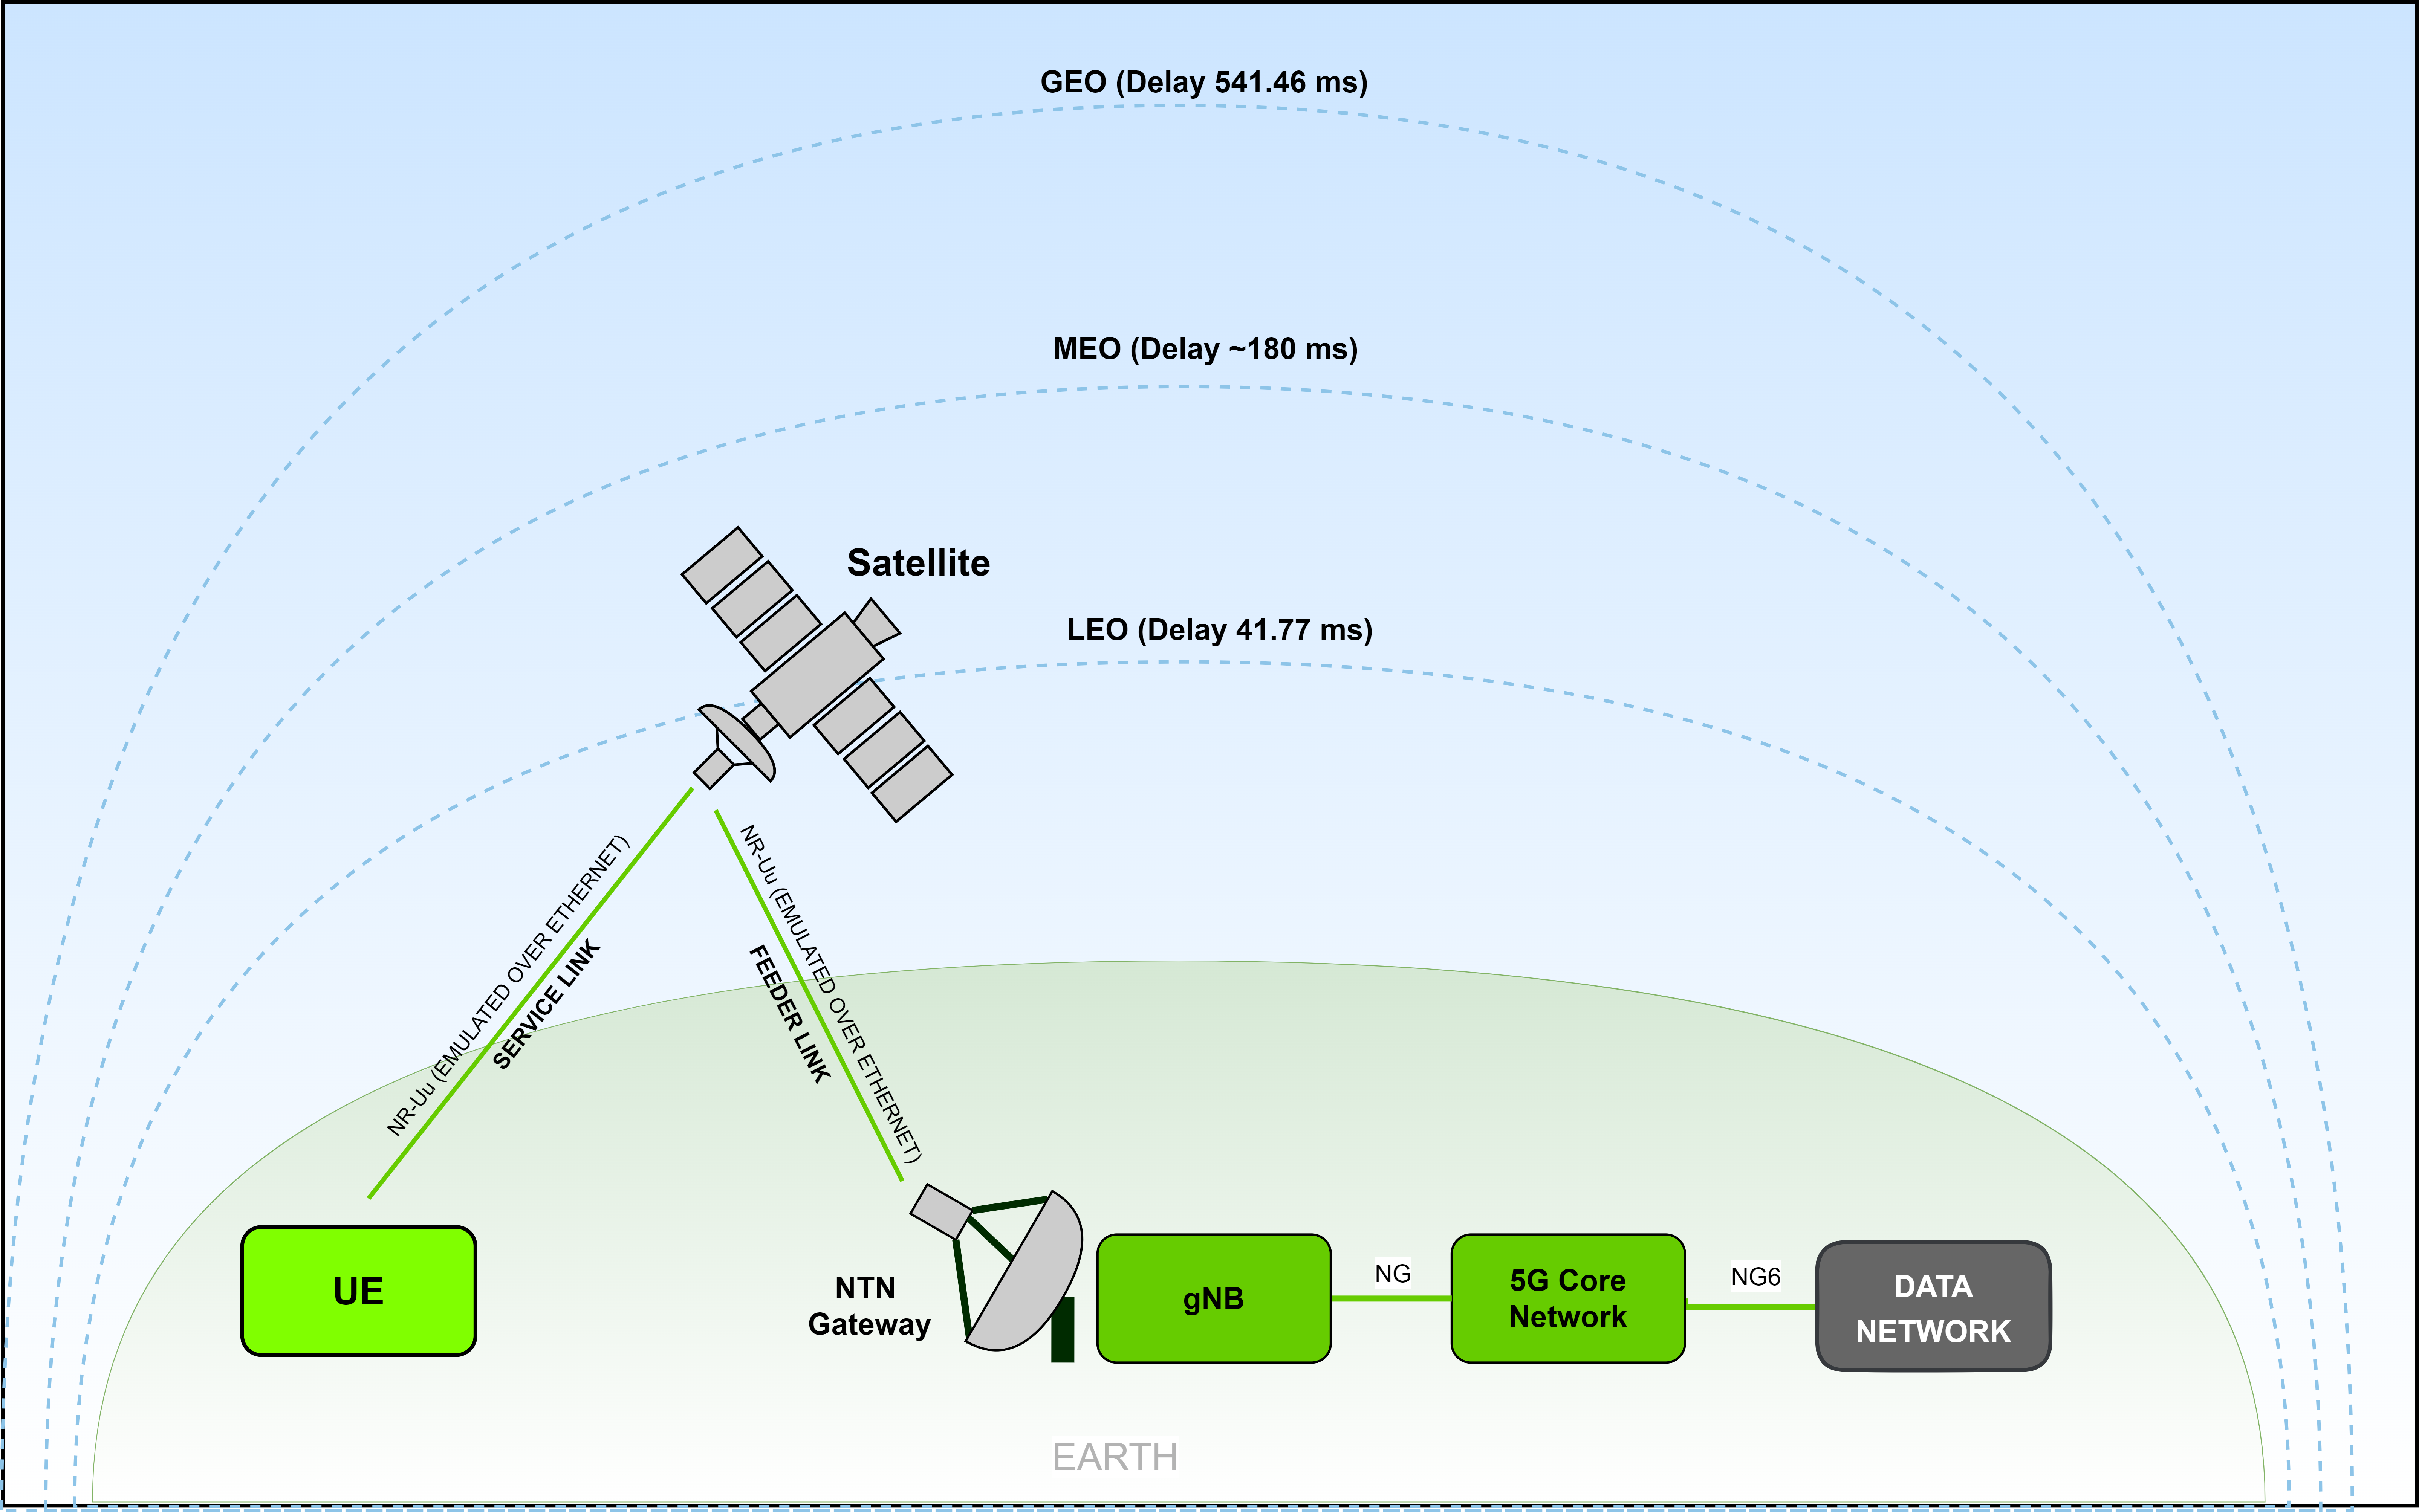
\includegraphics[width=\linewidth]{./figs/SATCOM_figure.png}
  		\caption{Transparent satellite based NG-RAN architecture}
  		\label{SATCOM_figure}
	\end{figure}
  
\end{frame} 


\section{Set-up for Demonstration of SATCOM}
\begin{frame}{Set-up for Demonstration of SATCOM}
    \begin{figure}[h!]
  		\centering
  		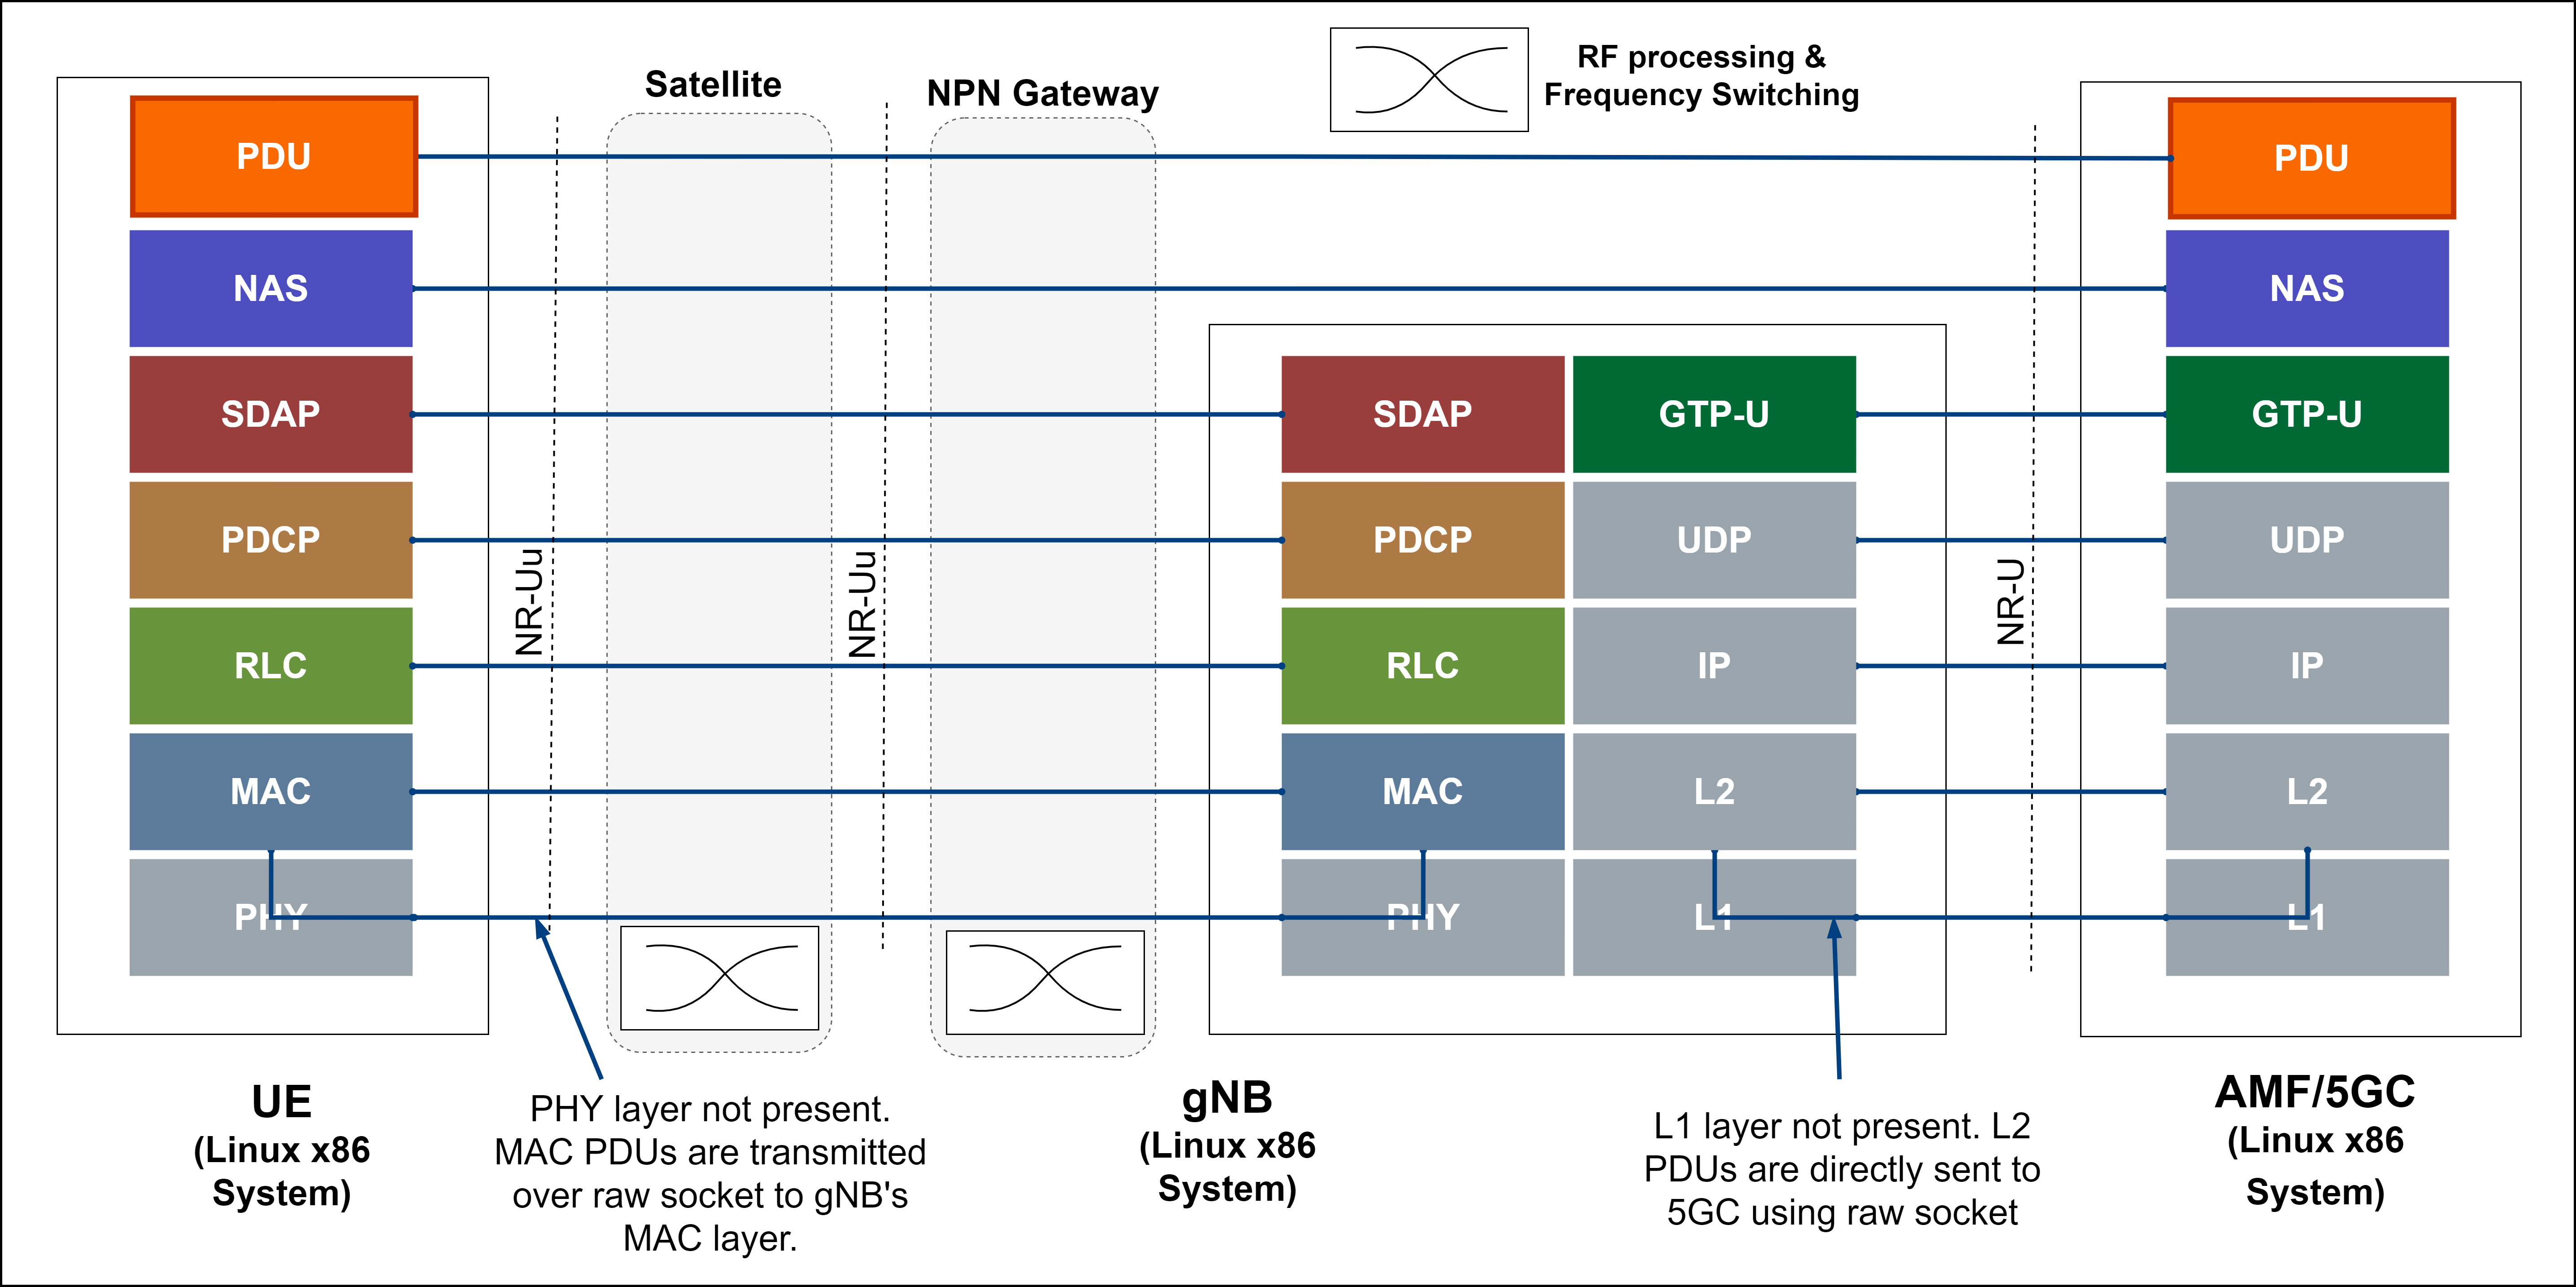
\includegraphics[width=\linewidth]{./figs/SATCOM_setup1.png}
  		\caption{Set-up for Demonstration of SATCOM}
  		\label{SATCOM_setup}
	\end{figure}
\end{frame} 

\section{Free-5GC Environment}
\begin{frame}{Free-5GC Environment}
	\begin{itemize}
    	\item The Free5GC project is an open-source initiative for mobile core networks of the fifth generation (5G) aimed  at construction of the 5G core network (5GC) as described in 3GPP Release 15 (R15) and futher.
    	\item It our setup it acts as our 5G core network and runs on a linux-x86 system to provides services to the UE via the gNB as defined by the 3GPP specifications.
    \end{itemize}

	\begin{figure}[h!]
  		\centering
  		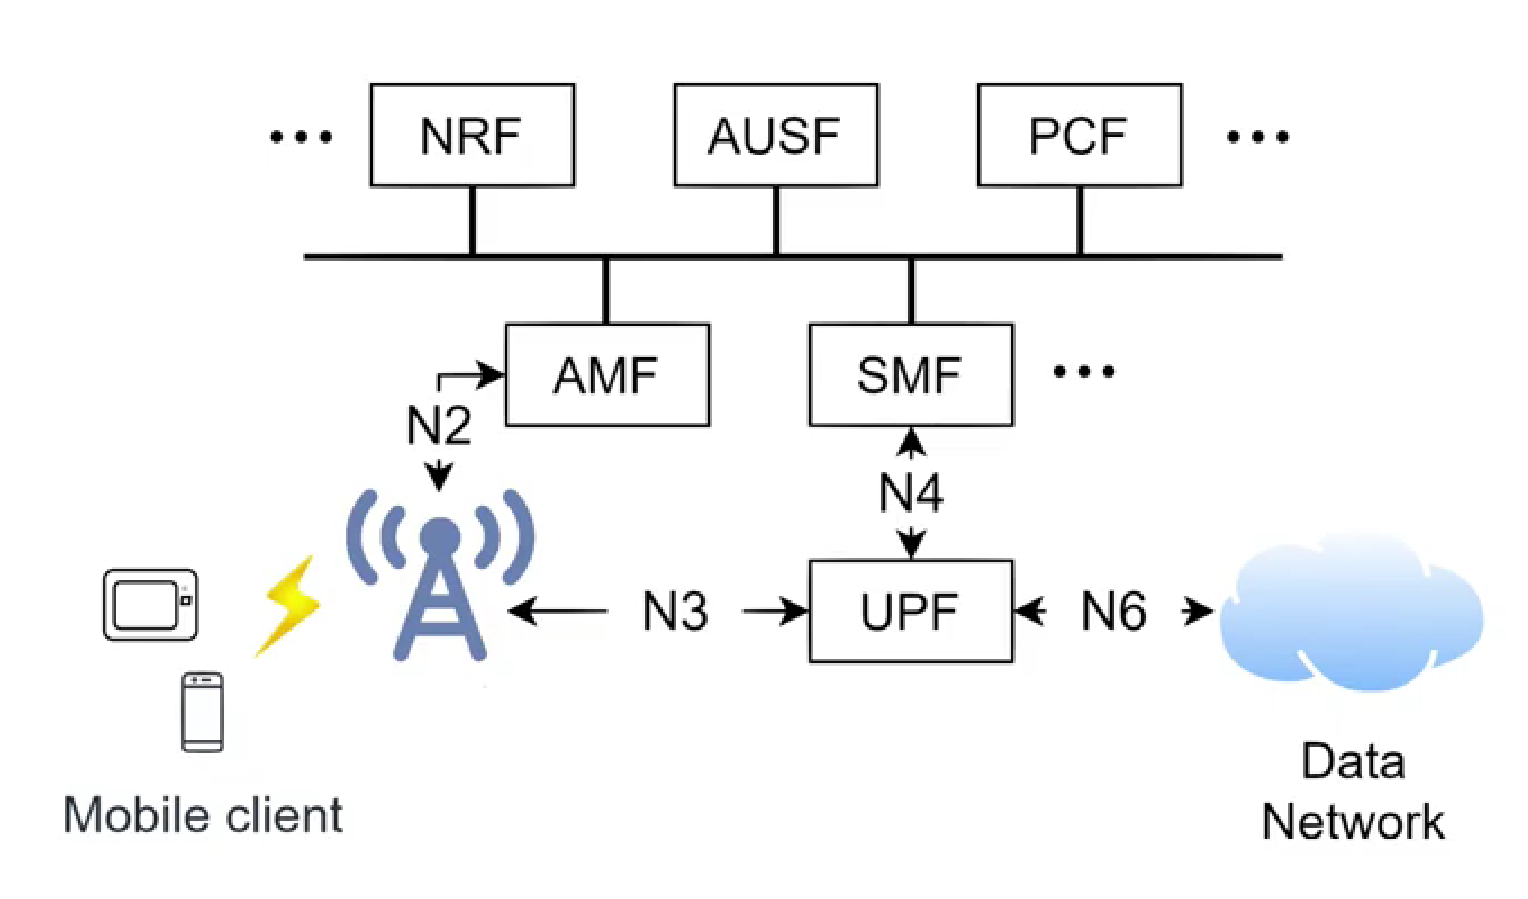
\includegraphics[width=0.7\linewidth]{./figs/Free5GC.png}
  		\caption{Free5GC Environment}
  		\label{Free5GC}
	\end{figure}
\end{frame} 

\section{Compilation and Execution at gNB}
\begin{frame}[fragile]{Compilation and Execution at gNB}
\begin{itemize}
    	\item Exporting environment variables for DPDK (Data Plane Development Kit consists of libraries to accelerate packet processing workloads):
\begin{lstlisting}
export RTE_SDK=<path to DPDK folder installed>
export RTE_TARGET=x86_64-native-linuxapp-gcc
\end{lstlisting}
	\item Loading Huge pages:
	\begin{lstlisting}
sudo su
echo 4096 > /sys/kernel/mm/hugepages/hugepages-2048kB/nr_hugepages
exit
\end{lstlisting}
\item Compiling and running the gNB App:
\begin{lstlisting}
cd ~/Documents/simran_wsp/bs_working/review-bs/5gnrps/src/gnbapp/test
make clean
make static -j10
sudo ./gnbapp enp1s0 -- -diersg
\end{lstlisting}
\end{itemize}
\end{frame}

\section{Compilation and Execution at UE}
\begin{frame}[fragile]{Compilation and Execution at UE}
\begin{itemize}
    	\item Exporting environment variables for DPDK (Data Plane Development Kit consists of libraries to accelerate packet processing workloads)
	\item Loading Huge pages
\item Compiling and running the gNB App:
\begin{lstlisting}
cd /home/greyteal/Documents/simran_wsp/UE/5gnrps/src/ueapp/test
make clean
make CPUSOC=1 JSON=1 -j10
sudo ./ueapp enp1s0 0 -- -dierns
\end{lstlisting}
\item Creating a tunnel interface for PDU session:
\begin{lstlisting}
sudo ifconfig tun00 10.60.0.1 up
sudo ip route add 192.168.134.224 dev tun00
\end{lstlisting}
\item Check the PDU session using ping (5 packets):
\begin{lstlisting}
ping -I tun00 192.168.134.224 -c 5
\end{lstlisting}
\end{itemize}
\end{frame}



\section{Emulating Satellite round-trip delay}
\begin{frame}[fragile]{Emulating Satellite round-trip delay}
\begin{itemize}
	\item A satellite in the GEO orbit has a round-trip signal delay of around 542ms.
	\item The entities in our setup communicate over LAN, hence we used a tool called NetEm to add the specified delay in our interface.
	\item NetEm allows linux user to add of delay, packet loss, duplication, and more to packets leaving a particular network interface.
	\item Fixed amount of delay:
	\begin{lstlisting}
sudo tc qdisc add dev enp2s0 root netem delay 542ms
\end{lstlisting}
\item Random delay:
	\begin{lstlisting}
sudo tc qdisc add dev enp2s0 root netem delay 542ms 20ms
\end{lstlisting}
\item Normal delay distribution:
	\begin{lstlisting}
sudo tc qdisc add dev enp2s0 root netem delay 542ms 20ms distribution normal
\end{lstlisting}
\end{itemize}
\end{frame}

\section{Testing the added latency using ping}
\begin{frame}
\frametitle{Testing the added latency using ping}
\begin{figure}[t!]
    \centering
    \begin{subfigure}[t]{0.5\textwidth}
        \centering
        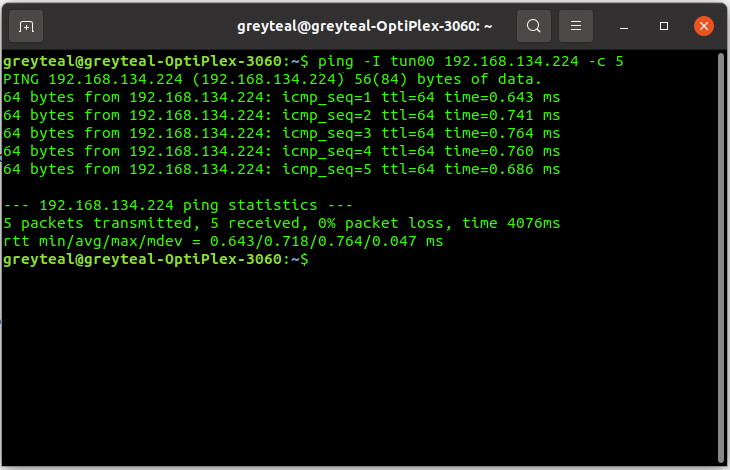
\includegraphics[width = 6cm]{./figs/Ping_before_adding_delay.png}
        \caption{Ping results before adding delay}
    \end{subfigure}%
    ~ 
    \begin{subfigure}[t]{0.5\textwidth}
        \centering
        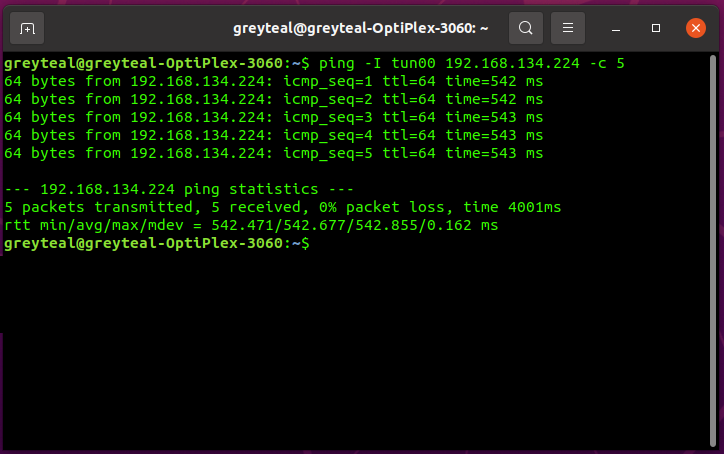
\includegraphics[width = 6cm]{./figs/Ping_after_adding_delay.png}
        \caption{Ping results after adding delay}
    \end{subfigure}
\end{figure} 	
\end{frame}


\section{5G-NR Call Flow}
\begin{frame}{5G-NR Call Flow as per 3GPP standards}
\begin{figure}[h!]
  		\centering
  		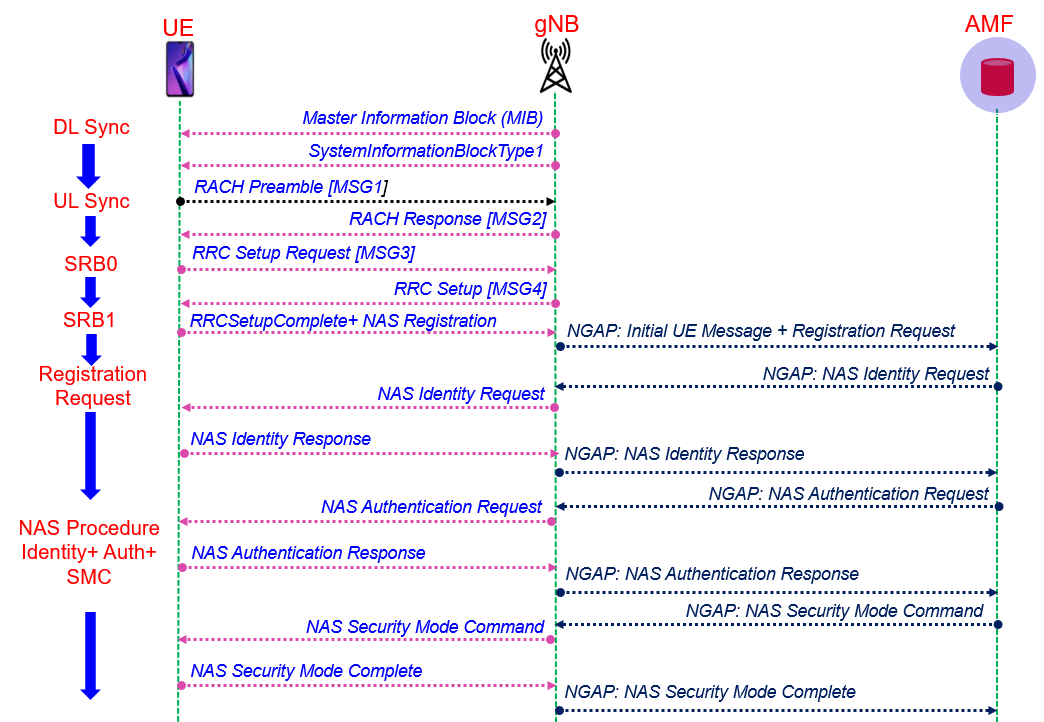
\includegraphics[width=0.8\linewidth]{./figs/5G_Call_Flow1.png}
  		\label{5G_Call_Flow1}
	\end{figure}
\end{frame}
\begin{frame}{5G-NR Call Flow as per 3GPP standards \small{(Continued)}}
\begin{figure}[h!]
  		\centering
  		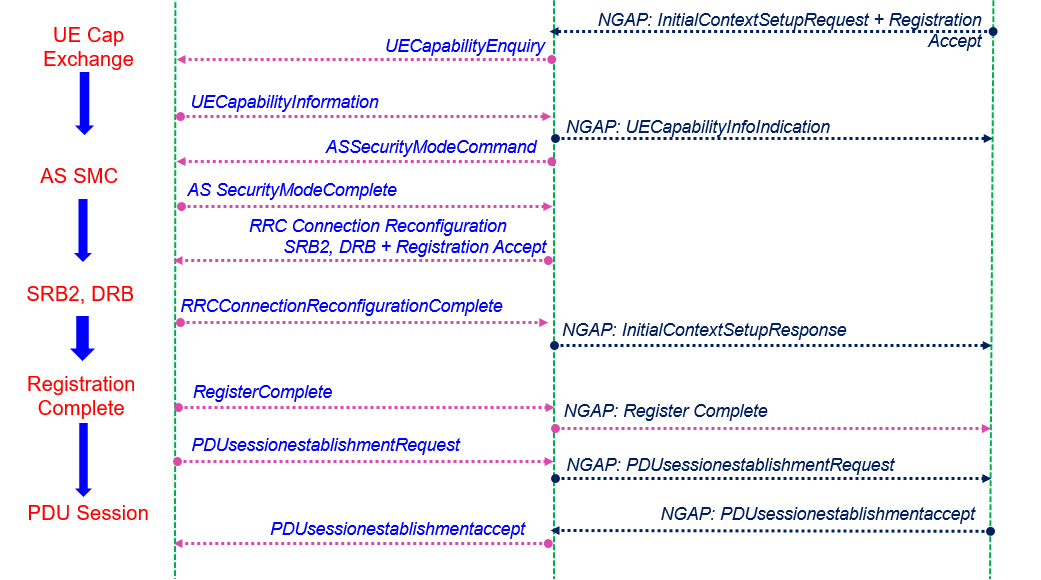
\includegraphics[width=0.8\linewidth]{./figs/5G_Call_Flow2.png}
  		\label{5G_Call_Flow2}
	\end{figure}
\end{frame}



\section{Streaming Video using the setup}
\begin{frame}[fragile]{Streaming Video using the setup}
\textbf{Creating video stream at source:}\\
\begin{itemize}
 \item 
 To create a video stream (using file videoplayback.mp4) from 5GC to UE via gNB, run the following command in terminal of 5GC workstation. This will use UDP to stream video to a given destination IP address and port number.\\
\begin{lstlisting}
cd ~/Documents #go to video path
vlc videoplayback.mp4 --sout=udp://10.60.0.1:1234
\end{lstlisting}
\end{itemize}
\end{frame}

\section{Streaming Video using the setup}
\begin{frame}[fragile]{Streaming Video using the setup \small{(Continued)}}
\textbf{Viewing video stream at the destination:}\\
\begin{itemize}
 \item The video packets streamed by source travel through the software stack as shown in Figure xx.
To view the stream at destination, run the following command in terminal. This will read the video packets received at the tun00 interface from the SDAP layer of software stack.\\
\begin{lstlisting}
vlc udp//@:1234 --miface=10.60.0.1:1234
\end{lstlisting}
\end{itemize}
\begin{figure}[h!]
  		\centering
  		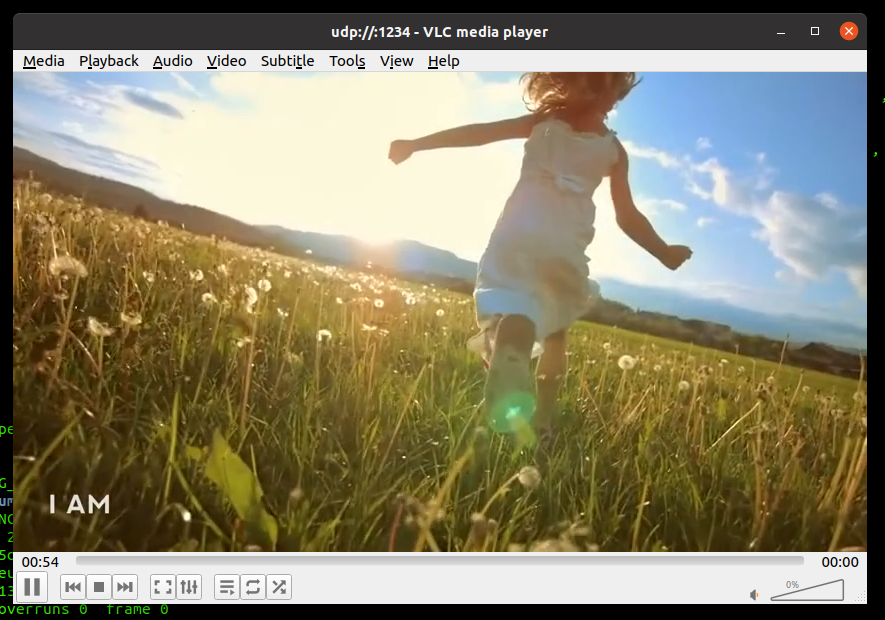
\includegraphics[width=0.5\linewidth]{./figs/Destination_viewing_stream.png}
  		\label{Destination_viewing_stream}
	\end{figure}
\end{frame}


\section{Video stream result}
\begin{frame}{Video stream result}
\begin{table}[]
\centering
\resizebox{0.9\textwidth}{!}{
\begin{tabular}{|c|c|c|}
\hline
\rowcolor[HTML]{DBDBEB} 
\textbf{Sr No.}                                                & \textbf{\begin{tabular}[c]{@{}c@{}}Delay between the play command \\ at source and video packets received \\ at the destination (sec)\end{tabular}} & \textbf{\begin{tabular}[c]{@{}c@{}}Delay between the stop command \\ at source and video packets halt at \\ the destination (sec)\end{tabular}} \\ \hline
1                                                              & 2.10                                                                                                                                                & 1.60                                                                                                                                            \\ \hline
2                                                              & 2.43                                                                                                                                                & 1.97                                                                                                                                            \\ \hline
3                                                              & 2.04                                                                                                                                                & 1.90                                                                                                                                            \\ \hline
4                                                              & 2.17                                                                                                                                                & 2.10                                                                                                                                            \\ \hline
5                                                              & 2.16                                                                                                                                                & 1.7                                                                                                                                             \\ \hline
\rowcolor[HTML]{E4E4EF} 
\multicolumn{1}{|l|}{\cellcolor[HTML]{E4E4EF}\textbf{Average}} & \textbf{2.18}                                                                                                                                       & \textbf{1.854}                                                                                                                                  \\ \hline
\end{tabular}
}
\caption{Result without ethernet delay}
\end{table}
\begin{table}[]
\centering
\resizebox{0.9\textwidth}{!}{
\begin{tabular}{|c|c|c|}
\hline
\rowcolor[HTML]{DBDBEB} 
\textbf{Sr No.}                                                & \textbf{\begin{tabular}[c]{@{}c@{}}Delay between the play command \\ at source and video packets received \\ at the destination (sec)\end{tabular}} & \textbf{\begin{tabular}[c]{@{}c@{}}Delay between the stop command \\ at source and video packets halt at \\ the destination (sec)\end{tabular}} \\ \hline
1                                                              & 2.78                                                                                                                                                & 2.57                                                                                                                                            \\ \hline
2                                                              & 2.58                                                                                                                                                & 2.32                                                                                                                                            \\ \hline
3                                                              & 2.69                                                                                                                                                & 2.42                                                                                                                                            \\ \hline
4                                                              & 2.64                                                                                                                                                & 2.74                                                                                                                                            \\ \hline
5                                                              & 2.85                                                                                                                                                & 2.43                                                                                                                                            \\ \hline
\rowcolor[HTML]{DBDBEB} 
\multicolumn{1}{|l|}{\cellcolor[HTML]{E4E4EF}\textbf{Average}} & \textbf{2.708}                                                                                                                                      & \textbf{2.496}                                                                                                                                  \\ \hline
\end{tabular}
}
\caption{Result with ethernet delay of 542 ms}
\end{table}
\end{frame}


\section{UGV control using NBIoT setup}
\begin{frame}{UGV control using NBIoT setup}
\begin{figure}[h!]
  		\centering
  		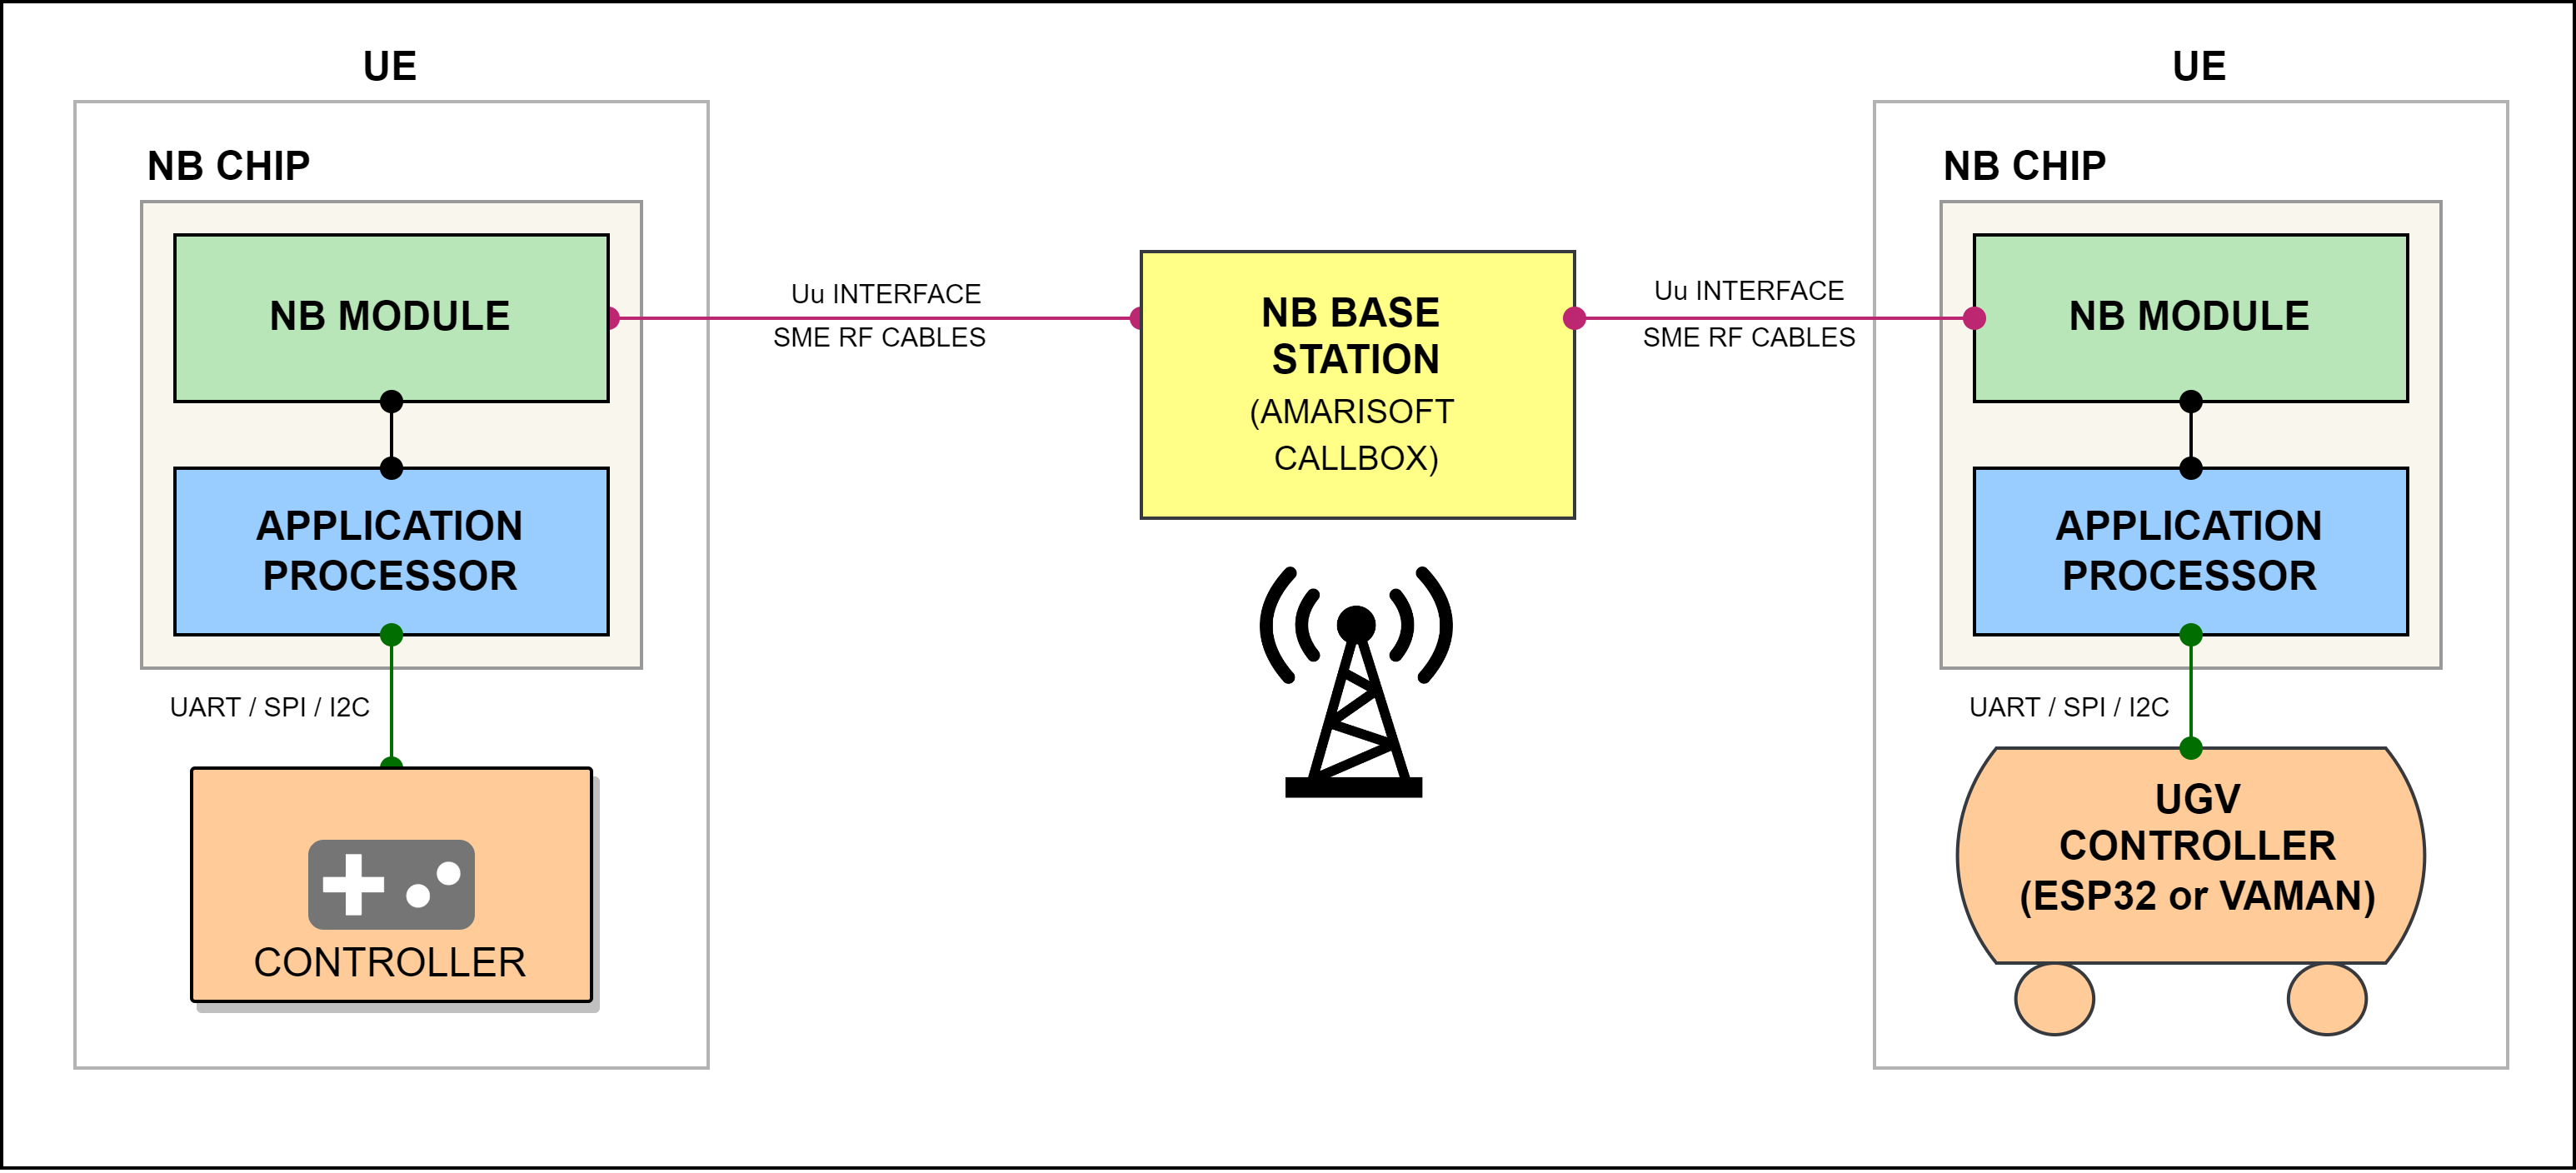
\includegraphics[width=\linewidth]{./figs/NBIoT_setup.png}
  		\label{NBIoT_setup}
  		\caption{UGV control using NBIoT setup}
\end{figure}

\end{frame}

\section{Conclusion}
\begin{frame}{Conclusion}
\begin{itemize}
 \item The basic principle behind motor control, use of serial interfaces (UART, SPI, I2C) and the inherent software remains similar to that of bigger sophisticated hardware of actual ground/aerial vehicle.
	\item Thus, The applications implemented on the UGV/UAV using ESP32/VAMAN can be scaled up to work on a real-life ground/aerial vehicle. This makes the UGV/UAV kit a good low cost prototype hardware.
	\item The 3GPP standards for Non-Terrestrial Network for 5G are only a couples of months away from their release, Thus the SATCOM infrastructure for 5G is not far from being commercial. 
	\item The experimental setup and results shown in this presentation confirms basic compatibility between satellite and 5G system.
	
\end{itemize}

\end{frame}

%\begin{frame}
%
%\begin{columns}
%\column{.5\textwidth}
%  \begin{itemize}
%  \item First item.
%  \item Second item.
%  \item Third item.
%  \end{itemize}
%\setbeamertemplate{itemize items}[square]
%  \begin{itemize}
%  \item First item.
%  \item Second item.
%  \item Third item.
%  \end{itemize}
%\column{.5\textwidth}
%\setbeamertemplate{itemize items}[circle]
%  \begin{itemize}
%  \item First item.
%  \item Second item.
%  \item Third item.
%  \end{itemize}
%\setbeamertemplate{itemize items}[ball]
%  \begin{itemize}
%  \item First item.
%  \item Second item.
%  \item Third item.
%  \end{itemize}
%\end{columns}
%
%\end{frame}



\begin{frame}[t,allowframebreaks]{References} 
	\nocite{*}
    \printbibliography
\end{frame}

\end{document}

